\documentclass[conference]{IEEEtran}
\IEEEoverridecommandlockouts
\usepackage{cite}
\usepackage{amsmath,amssymb,amsfonts}
\usepackage{algorithmic}
\usepackage{graphicx}
\usepackage{textcomp}
\usepackage{xcolor}
\usepackage{siunitx}
\usepackage{hyperref}
\usepackage{upgreek}
\def\BibTeX{\rm B\kern-.05em{\sc i\kern-.025em b}\kern-.08em
    T\kern-.1667em\lower.7ex\hbox{E}\kern-.125emX}

\begin{document}

\title{Development and Characterization of a Gold-Bump Flip-Chip Bonding Process for RF IC Applications\\
\thanks{This paper is written as part of a Bachelor of Electrical Engineering project in the Department of Integrated Circuits of the TU/e, in the period of 2025-02-13 to 2025-06-11 and was supervised by M. Fattori, G. Radulov, T. Matray and assisted by V. Vidojkovic and V. Zaoutis.}
}

\author{\IEEEauthorblockN{Daniel Tyukov}
\IEEEauthorblockA{Integrated Circuits Group, Department of Electrical Engineering\\
Eindhoven University of Technology\\
Eindhoven, The Netherlands\\
d.tyukov@student.tue.nl}}

\maketitle
\thispagestyle{plain}
\pagestyle{plain}

\begin{abstract}
Gold-stud-bumped flip-chip interposers on glass promise the low-parasitic links needed in next-generation RF system-in-package (SiP) assemblies, yet existing research often relies on multilayer metal stacks and complex bonding profiles. This work demonstrates a simplified alternative: a single layer \(\mathrm{Ti}/\mathrm{Au}\) Ground-Signal-Ground (GSG) coplanar waveguide (CPWG) interposer that is joined to silicon Integrated Circuit chips through \(70\,\upmu\text{m}\) thermosonic placed gold stud bumps. The process covers bump formation, flip-chip thermo-compression, and open-short de-embedding. Broadband electrical measurements are summarized into two compact circuit elements: (i) a lumped bump model that behaves as a simple series resistance in the low-megahertz range and (ii) a \(\pi\)-model for the on-interposer GSG transmission lines. The high interconnect yield and verified models can be inserted directly into a process design kit, enabling cost-effective RF SiP prototypes on glass substrates.
\end{abstract}

\begin{IEEEkeywords}
flip-chip bonding, gold stud bumps, Ti/Au CPWG interposer, thermosonic bonding, RF SiP, lumped modeling, de-embedding, yield characterization
\end{IEEEkeywords}

\IEEEpeerreviewmaketitle

\section{Introduction}
Flip-chip integration replaces the millimeter-long wires of conventional wire bonding with micrometer-scale metallic bumps, thus reducing parasitic inductance and extending the useful bandwidth of radio frequency (RF) links well beyond \SI{10}{\giga\hertz}.  The geometric contrast is visualized in Fig.~\ref{fig:flipchip_vs_wirebond}: a wire-bonded die must loop current over the pad edge, whereas a flip-chipped die conducts directly through the bump into the interposer.  Thanks to this topological advantage, the technique is now standard for high-speed processors and is being explored for heterogeneous System-in-Package (SiP) assemblies targeting mm-wave and broadband applications \cite{Lau2016,Heinrich2005}.

State-of-the-art demonstrators typically rely on multilayer ceramic or silicon carriers in combination with solder-based controlled-collapse chip connection (C4) bumps.  Although these stacks deliver excellent RF performance, they require expensive thin-film processing and dedicated bumping lines.  Glass substrates have emerged as an attractive alternative due to their low permittivity, panel-level scalability, and a custom-made thermal expansion coefficient (CTE) \cite{Keech2013}.  In parallel, thermosonic (TS) gold (Au) stud bumps offer a solder-free option that avoids under-bump metallurgy and reflow cycles.  Recent work has optimized the bump distribution for TS bonding \cite{Chang2022}, proposed high-reliability Au–Au pad strategies \cite{Yan2024}, and demonstrated Au-stud flip-chip assemblies that operate up to \SI{600}{\celsius} in Stacking integrated Circuits (SiC) \cite{Li2024}.  However, quantitative RF data for Au studs on single-layer glass interposers, together with statistically meaningful yield figures, remain an under-researched field of study.

This study addresses this gap by developing a simple and fully in-house integration flow that combines a glass interposer patterned with a single \SI{50}{\nano\metre}/\SI{100}{\nano\metre} Ti/Au metal layer, \SI{70}{\micro\metre} with TS Au studs deposited using a standard wire-bonding process. Next, flip-chip bonding based on thermo-compression will be used to connect the die to the interposer.  This whole process can be performed within TU/e facilities. The work further investigates three main research questions: (i) How can the electrical behavior of a single Au stud bump on glass be captured by a low-frequency lumped model? (ii) How well does a closed-form $\pi$-model predict the performance of a single-metal coplanar waveguide on glass between \SI{10}{\mega\hertz} and \SI{10}{\giga\hertz}? (iii) Which process parameters delivers an acceptable bump-bond yield without damaging thin RF dies and interposer metallization layer in the process?

The remainder of the paper is organized as follows. Section \ref{sec:model} develops the analytical and \textsc{qucs}-based circuit simulation models that guided the design of the interposer mask in \textsc{klayout}. Section \ref{sec:fabrication} details bump formation, flip-chip bonding, and sample examination, emphasizing the process window accessible with standard equipment. Experimental RF and yield results are presented and discussed in Section~\ref{sec:results}. Section \ref{sec:results} also summarizes the findings and outlines future directions toward broadband RF SiP demonstrators.

\begin{figure}[htbp]
\vspace{-8px}
  \centering
  \begin{minipage}[t]{0.49\linewidth}
    \centering
    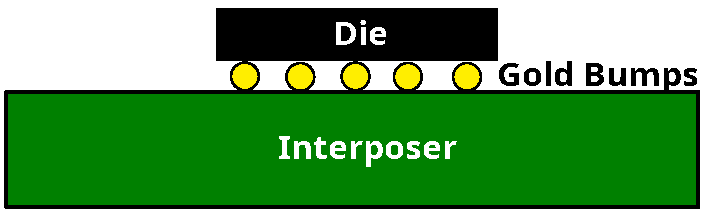
\includegraphics[width=\linewidth]{figures/flipchip2.pdf}\\
    (a)
  \end{minipage}\hfill
  \begin{minipage}[t]{0.49\linewidth}
    \centering
    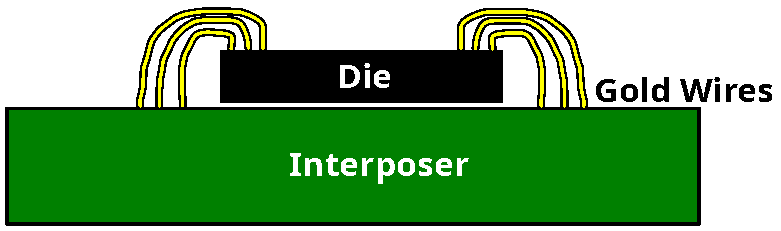
\includegraphics[width=\linewidth]{figures/wirebond2.pdf}\\
    (b)
  \end{minipage}
  \caption{IC integration approaches: (a) flip-chip and (b) wire-bonding.}
  \label{fig:flipchip_vs_wirebond}
  
\end{figure}


\section{Modeling and Simulation of Expected Results}\label{sec:model}

\subsection{Bump--Line Model Simulation}\label{subsec:bump_line_model}

The electrical link between the transceiver front-end (TXFE) die and the single-metal glass interposer consists of three thermosonically placed gold bumps that land on a GSG trace ends acting like pads. The design is shown in Fig.~\ref{fig:interposer_layouts} for the mask of the interposer and Fig.~\ref{fig:vna_setup}(a) for the microscope image of the GSG trace. The central bump carries the signal, while the two side bumps are ground.  This topology is abstracted by placing the lumped impedance of one signal bump in series with two parallel ground bumps in series with the CPWG GSG trace and finally terminating the network with the measured S-parameter file of the TXFE die. The complete one-port model is implemented in \textsc{qucs} Fig.~\ref{fig:qucs}. Its simulated response is later compared with the de-embedded measurement in Fig.~\ref{fig:sim_real}.

The dimensions and values used in the calculations are listed in Table.~\ref{tab:cpwg_params}, every symbol that appears in the equations below can be cross-referenced there. All formulations are obtained from \cite{Simons2004}. The thick glass quasi-TEM effective permittivity is

\begin{equation}
\varepsilon_{\text{eff}}=\frac{\varepsilon_{r}+1}{2}=4.375,
\label{eq:eps_eff}
\end{equation}

and the even-mode filling factor is

\begin{equation}
k=\frac{w}{w+2s}=0.456,\qquad
k'=\sqrt{1-k^{2}}.
\label{eq:k_factor}
\end{equation}

These values give the characteristic impedance.

\begin{equation}
Z_{0}=\frac{30\pi}{\sqrt{\varepsilon_{\text{eff}}}}\,
      \frac{K(k')}{K(k)}=\SI{49.8}{\ohm},
\label{eq:Z0}
\end{equation}

where \(K(\cdot)\) is the complete elliptic integral. The per-unit-length elements of the line are then

\begin{subequations}\label{eq:cpwg_pul}
\begin{align}
R'&=\frac{\rho}{w\,t}=4.82\times10^{-3}\ \Omega/\si{\micro\metre},\\
C'&=\frac{\sqrt{\varepsilon_{\text{eff}}}}{Z_{0}c}=1.15\times10^{-16}\ \mathrm{F}/\si{\micro\metre},\\
L'&=Z_{0}^{2}C'=4.23\times10^{-13}\ \mathrm{H}/\si{\micro\metre},\\
G'&=\omega C'\tan\delta=3.61\times10^{-11}\ \mathrm{S}/\si{\micro\metre}
     \;\;(@\SI{10}{\mega\hertz}),
\end{align}
\end{subequations}

which, when multiplied by the physical length of the GSG traces \(\ell=\SI{1.15}{\milli\metre}\), yield the $\pi$-model of Fig.~\ref{fig:qucs}: \(R=\SI{5.54}{\ohm}\), \(L=\SI{0.486}{\nano\henry}\) and \(C_{1}=C_{2}=\SI{66.1}{\femto\farad}\). Comparable impedances for single-metal glass interposers were reported in  \cite{Wang2016}. These analytic estimates will be compared with the results of the de-embedding process section \ref{subsec:rlcg}.

Each gold stud begins as a \SI{25}{\micro\metre} wire and is coined into a bump of nominal diameter \(D_{\text{b}}=\SI{70}{\micro\metre}\) (radius \(r_{\text{b}}=\SI{35}{\micro\metre}\)) and height \(h_{\text{b}}=\SI{25}{\micro\metre}\). Using the lumped parameter equations from \cite{Simons2004} of a single bump, the calculations are as follows.

\begin{subequations}\label{eq:bumps_single}
\begin{align}
R_{\text{b}}&=\frac{\rho h_{\text{b}}}{\pi r_{\text{b}}^{2}}=\SI{2.29}{\milli\ohm},\\
L_{\text{b}}&=\mu_{0}h_{\text{b}}\!\left[\ln\!\left(\tfrac{4h_{\text{b}}}{r_{\text{b}}}\right)+1\right]=\SI{64}{\pico\henry},\\
C_{\text{b}}&=\frac{\varepsilon_{0}\varepsilon_{\text{eff}}\pi r_{\text{b}}^{2}}{s}
             =\SI{3.6}{\femto\farad}.
\end{align}
\end{subequations}

When the three bumps are combined, the two grounds appear in parallel and the resulting impedance is \(Z_{\text{3b}}=\tfrac{3}{2}Z_{\text{b}}\).  The resistance therefore decreases to \(R_{\text{3b}}=\SI{0.24}{\milli\ohm}\) because the ground current splits between two paths, the inductance increases to \(L_{\text{3b}}=\SI{96}{\pico\henry}\) because the magnetic fluxes of the series elements increase, and the pad-to-substrate capacitance remains essentially the same, \(C_{\text{3b}}=\SI{3.6}{\femto\farad}\).

The complete one-port thus consists of the measured TXFE die, the three-bump transition, and the GSG trace. After fabrication and characterization it will serve as a reference against which the de-embedded measurement in Fig.~\ref{fig:sim_real} will be benchmarked.


\begin{table}[htbp]
\vspace{-8px}
  \caption{CPWG design parameters on glass substrate}
  \label{tab:cpwg_params}
  \centering
  \begin{tabular}{|c|l|c|}
    \hline
    \textbf{Symbol} & \textbf{Meaning} & \textbf{Value} \\ \hline
    $w$              & Signal-strip width                 & \SI{69}{\micro\metre} \\ \hline
    $s$              & Signal–ground gap                  & \SI{41}{\micro\metre} \\ \hline
    $g$              & Ground-bar width                   & \SI{153}{\micro\metre} \\ \hline
    $t$              & Metal thickness (Ti/Au)            & \SI{150}{\nano\metre} \\ \hline
    $\rho$           & Sheet resistivity (measured)       & \SI{4.99e-8}{\ohm\metre} \\ \hline
    $\varepsilon_r$  & Relative permittivity of glass     & 7.75 \\ \hline
    $\tan\delta$     & Loss tangent                       & 0.005 \\ \hline
    $\ell$           & Physical length                    & \SI{1.15}{\milli\metre} \\ \hline
  \end{tabular}
\end{table}

\begin{figure}[htbp]
  \centering
\vspace{-8px}  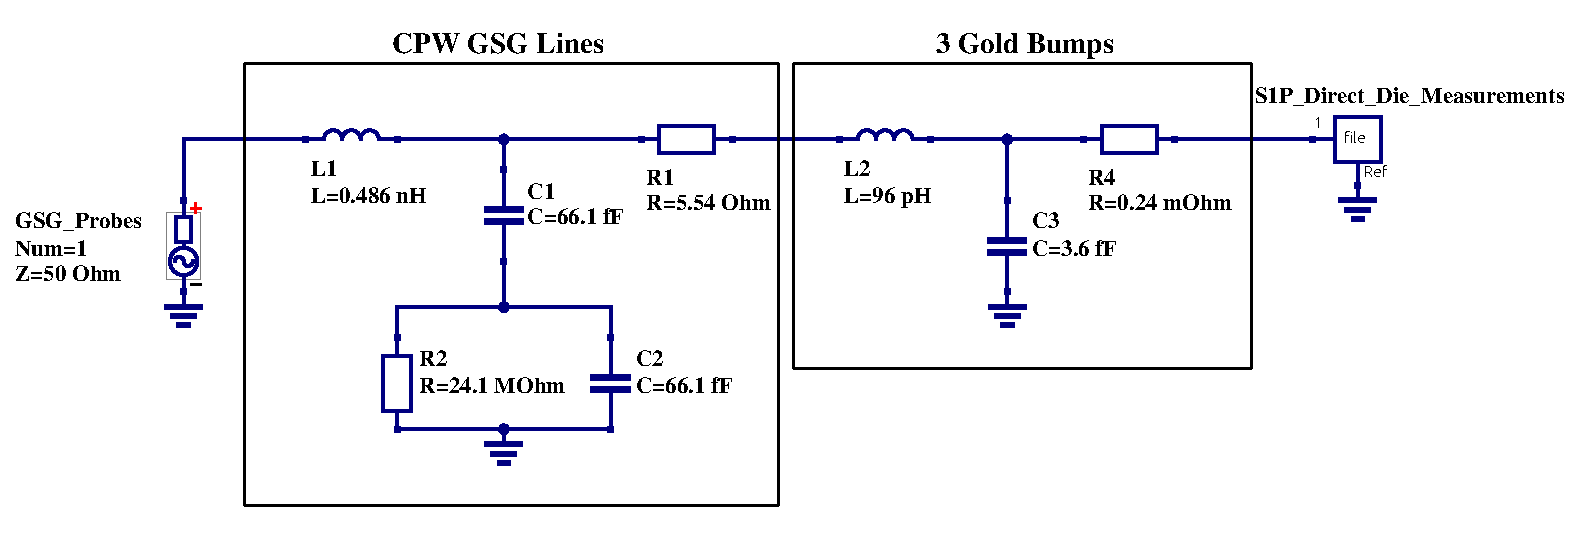
\includegraphics[width=\linewidth]{figures/rf_simulated_dut_qucs_circuit_final.pdf}
  \caption{One-port \textsc{qucs} schematic comprising the CPWG
  \(\pi\)-model, the three-bump transition and the measured
  \texttt{*.s1p} file of the TXFE die.}
  \label{fig:qucs}
    \vspace{-10px}
\end{figure}

\begin{figure}[htbp]
\vspace{-8px}
  \centering
  \begin{minipage}[t]{0.49\linewidth}
    \centering
    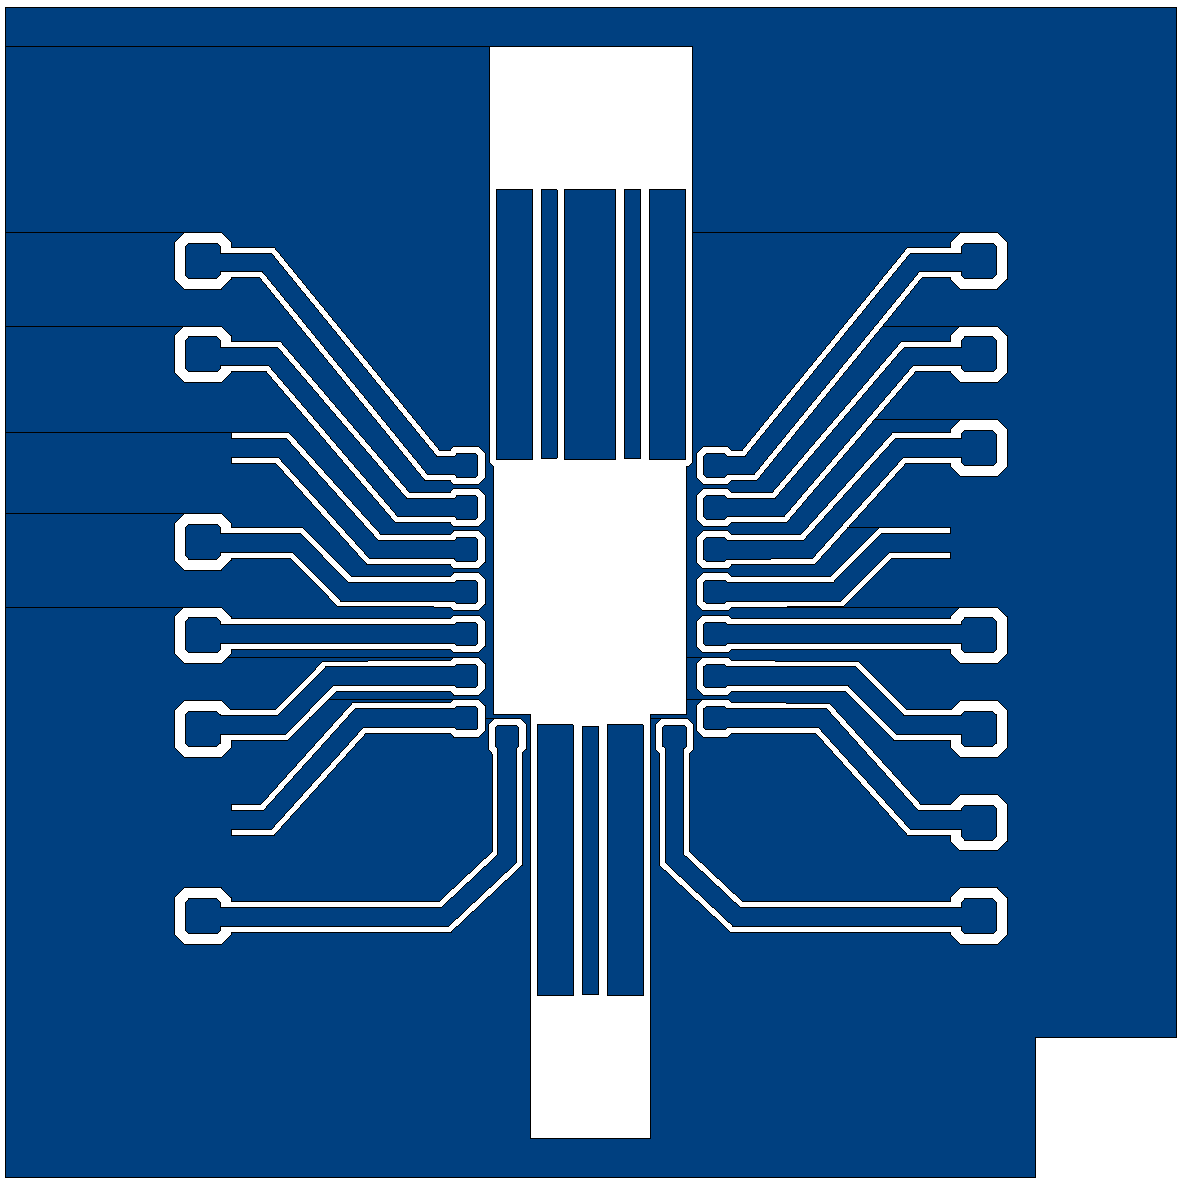
\includegraphics[width=0.8\linewidth]{figures/rf_layout_thru.png}\\
    (a)
  \end{minipage}\hfill
  \begin{minipage}[t]{0.49\linewidth}
    \centering
    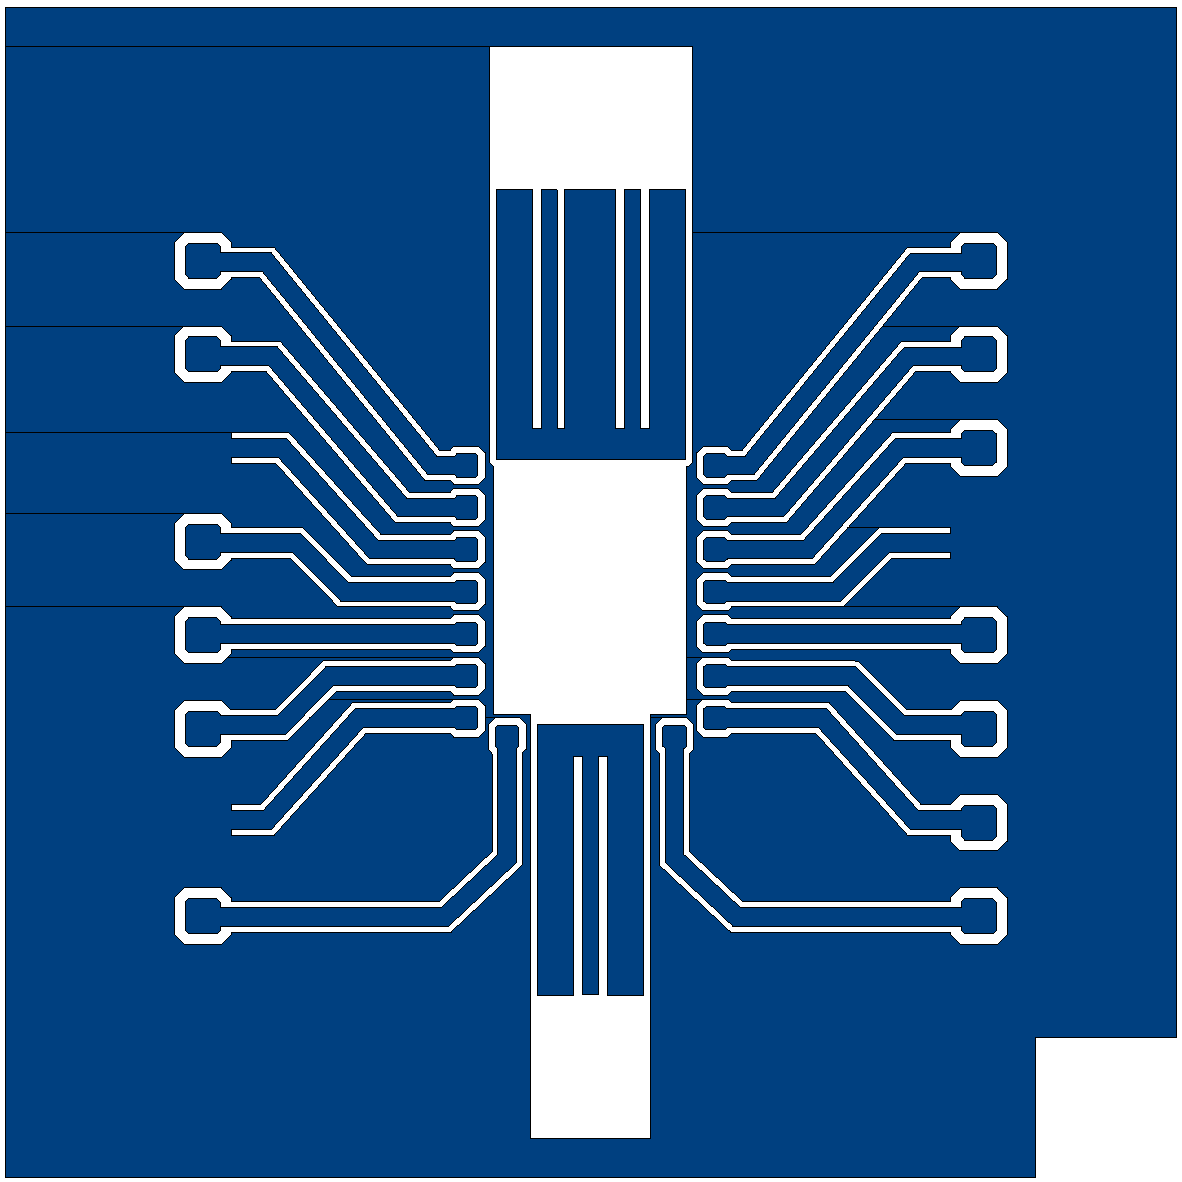
\includegraphics[width=0.8\linewidth]{figures/rf_layout_reflect.png}\\
    (b)
  \end{minipage}
  \caption{Interposer calibration structures used for one-port
  de-embedding: (a)~REFLECT and (b)~THROUGH–OPEN.}
  \label{fig:interposer_layouts}
  \vspace{-10px}
\end{figure}

\subsection{Yield-Test Structure Simulation}\label{subsec:yield_sim}

The goal of the yield-test interposer is to characterize the
thermosonic bump bond process before fabricating the RF
interposer.  Fig.~\ref{fig:yield_3d_2d}(b) shows the single-metal glass
interposer mask overlaid with the second interposer with blue lines that will be flipped onto it and carries \(N_{\mathrm{line}}=24\) striplines. A dummy die, patterned with the same Ti/Au stack, mirrors the pad
geometry and is flipped on top Fig.~\ref{fig:yield_3d_2d}(a).  After
bonding, every line is ideally shorted by a \(D_{\mathrm{b}}=\SI{70}{\micro\metre}\) gold stud bump; missing or bridged bumps therefore count as open or parallel short circuits in DC. The probe pads touch the two ends of the interposer, allowing continuity measurements on a multimeter.

The analysis follows \cite{Ullan2004}, treating open and short defects as independent rare events.  
Let \(\lambda_{\mathrm{op}}\) and \(\lambda_{\mathrm{sh}}\) be the
probabilities that one bond is, respectively, open or shorted.  The
probability of defective bond total is
\(\lambda=\lambda_{\mathrm{op}}+\lambda_{\mathrm{sh}}\).
The calculations are performed in section \ref{subsec:yield_res}.

\begin{figure}[htbp]
  \centering
  \begin{minipage}[t]{0.49\linewidth}
    \centering
    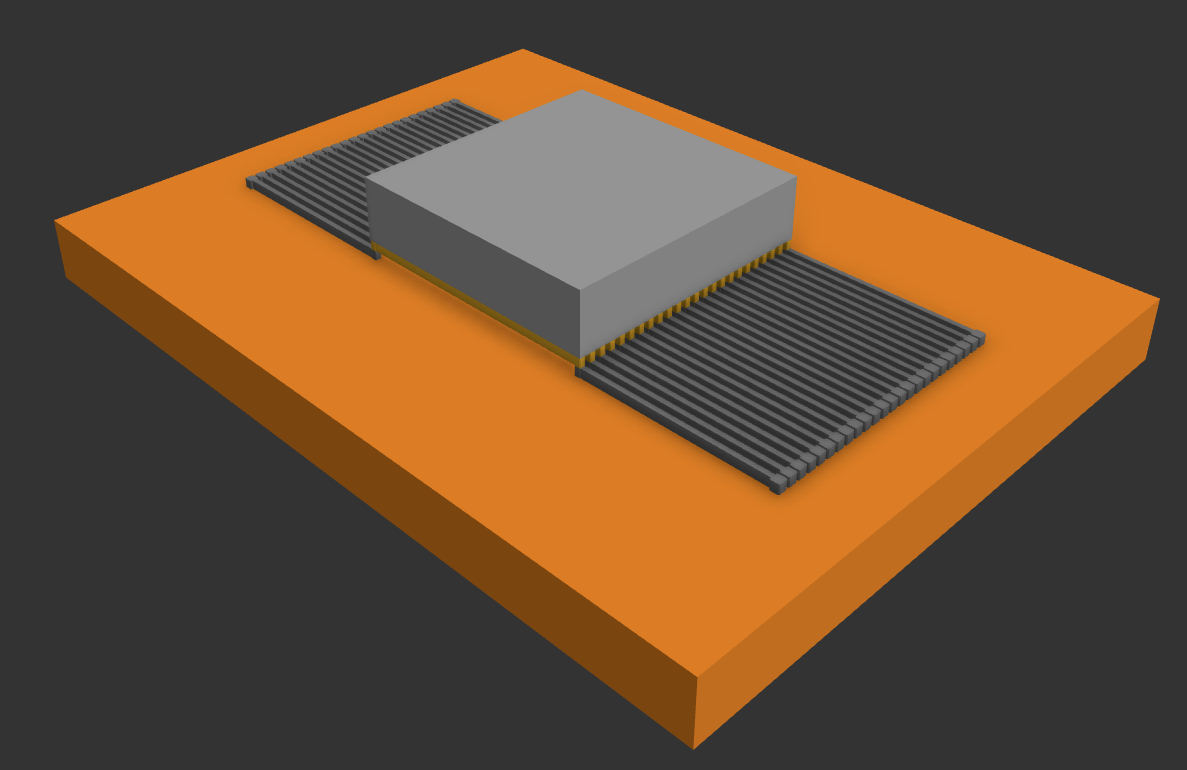
\includegraphics[width=\linewidth]{figures/yield_test_fake_die.png}\\
    (a)
  \end{minipage}\hfill
  \begin{minipage}[t]{0.49\linewidth}
    \centering
    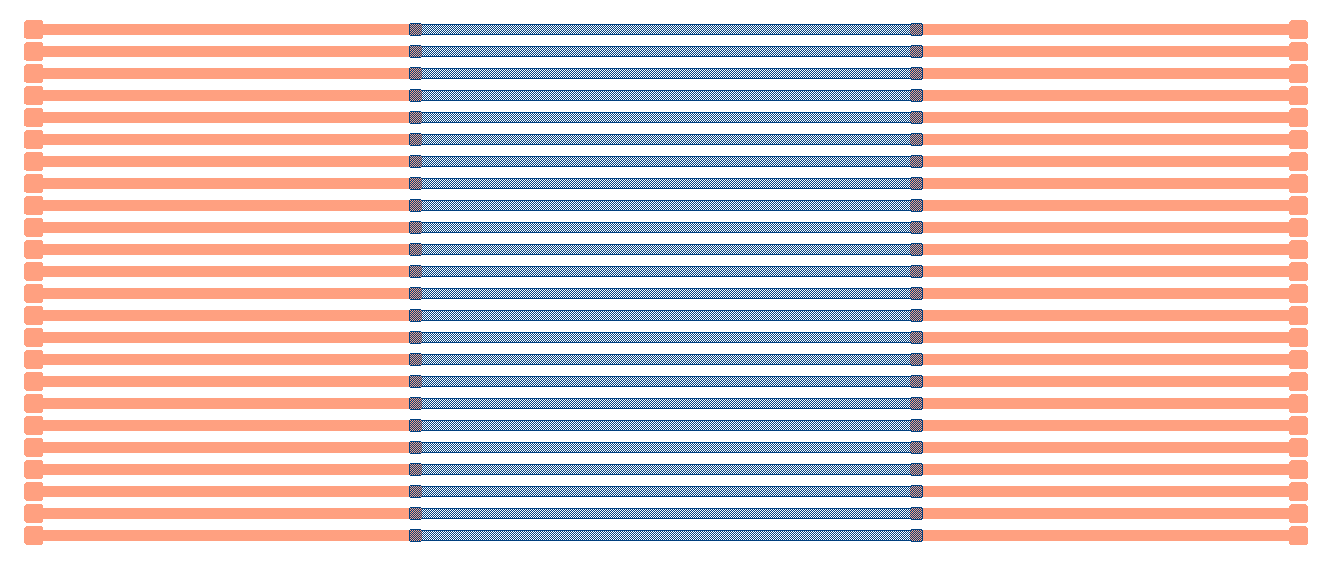
\includegraphics[width=\linewidth]{figures/yield_layout.png}\\
    (b)
  \end{minipage}
  \caption{3-D visualizations of the yield-test assembly:
  (a) dummy die flip-chipped onto the interposer,
  (b) 2-D mask of the yield-test interposer (orange) overlaid with the
  dummy die (blue) that will be flip-chipped on top. Each of the
  24 striplines terminates in probing pads.}
  \label{fig:yield_3d_2d}
    \vspace{-10px}
\end{figure}

\section{Fabrication and Measurement}\label{sec:fabrication}

\subsection{Assembly Flow Overview}\label{subsec:flow}

Fig.~\ref{fig:interposer_flow} condenses the complete sequence from mask design to RF testing. Masks are made in \textsc{klayout} and transferred to a glass substrate. A negative photoresist lift-off process defines the single-metal pattern; a \SI{50}{\nano\metre}/\SI{100}{\nano\metre} Ti/Au stack is then evaporated and lifted off to produce the conductive traces that make up the interposer. Gold stud bumps with a diameter of \SI{70}{\micro\metre} are placed on the interposer pads with a TPT HB16 bonder (\SI{250}{mN}, \SI{500}{ms}, \SI{150}{\celsius}). After visual inspection, the bumped carrier is cleaned, aligned with a GaN TXFE die, and thermo-compressed on a Dr. Tretsky T-5300. Electrical continuity is verified at room temperature before the assembly proceeds to extracting S-parameters for open-short de-embedding on an MPI THz selection probe station equipped with \(\lvert Z\rvert\) GSG probes and a Keysight PNA-X N5247B vector network analyzer.  

\begin{figure}[htbp]
  \centering
  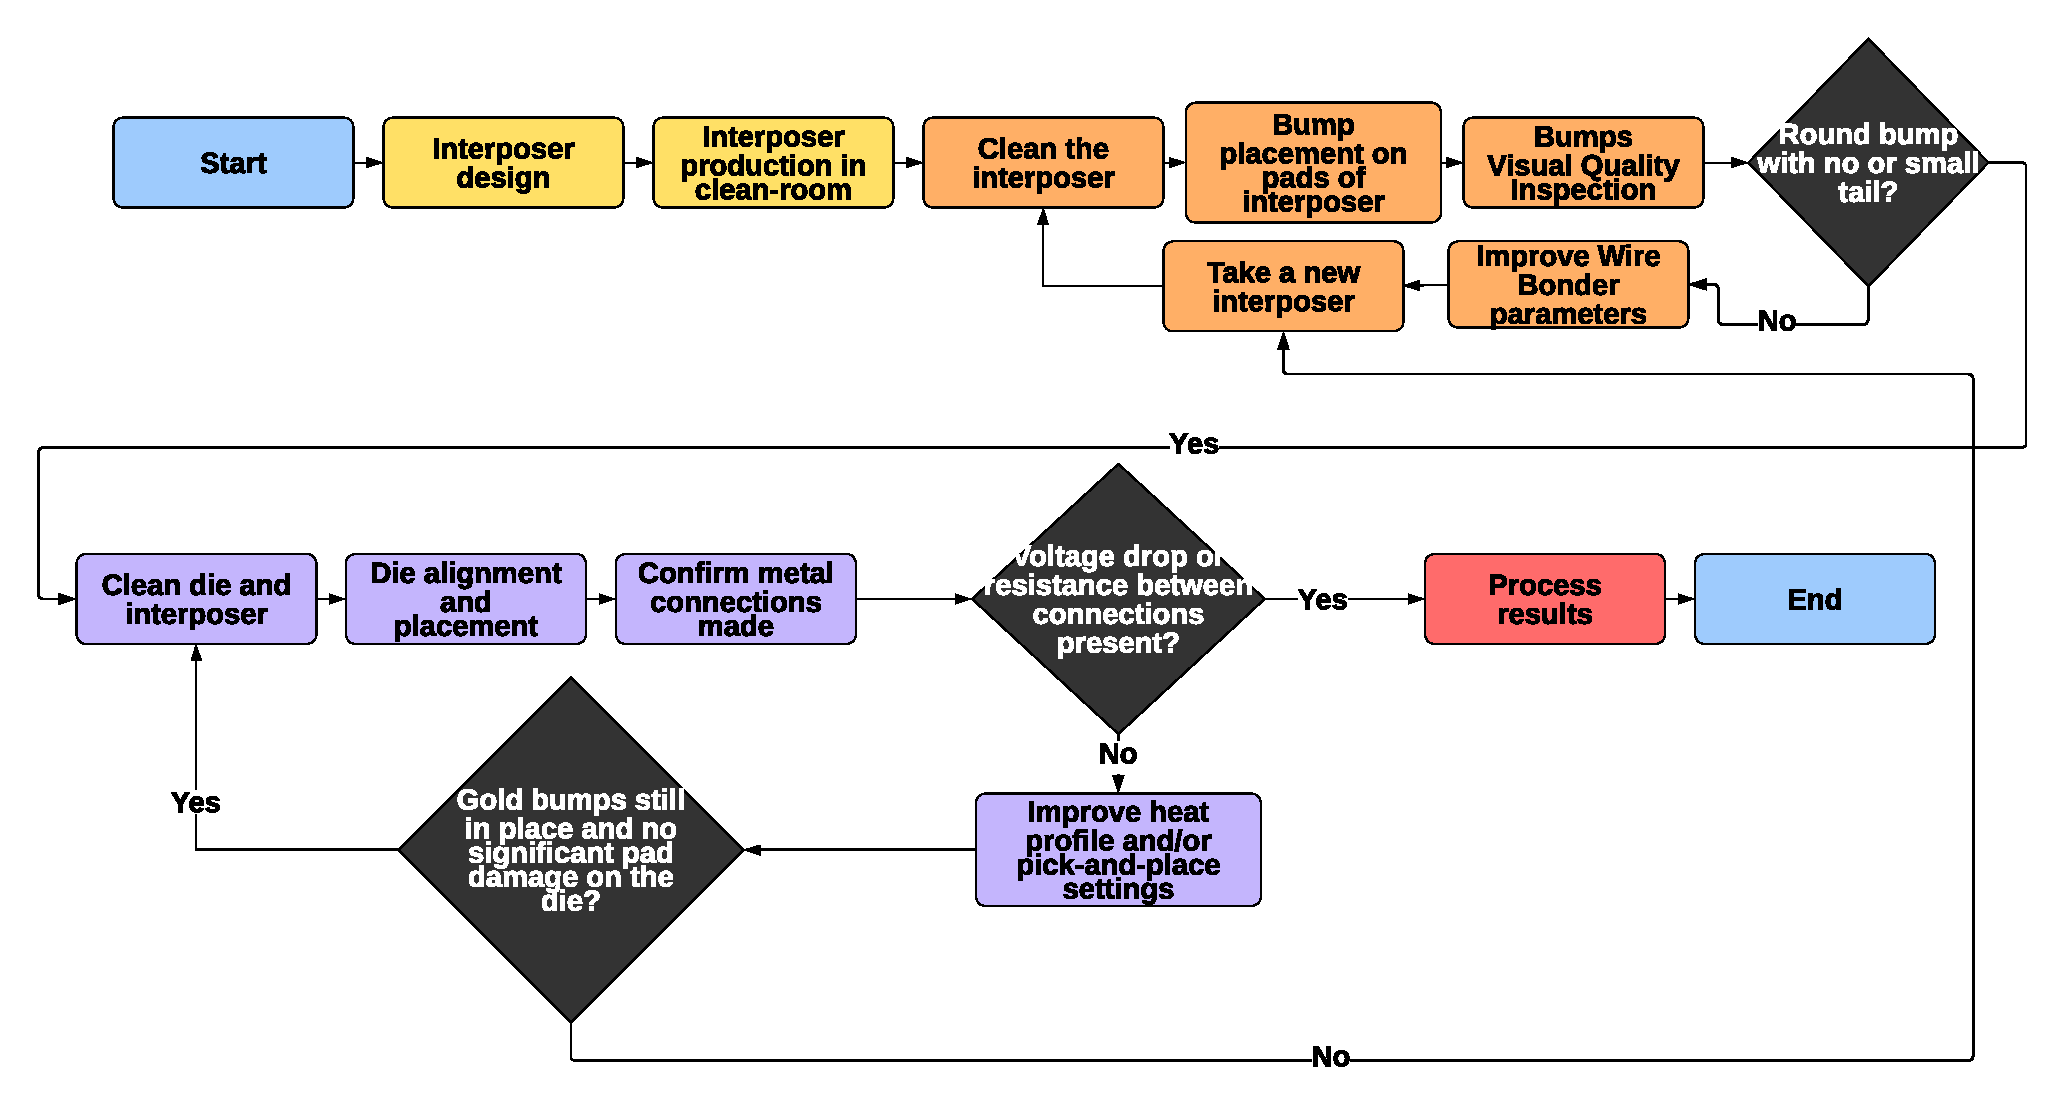
\includegraphics[width=\linewidth]{figures/interposer_flowchart2.pdf}
  \caption{Process flow from interposer design to RF-tested flip-chip assembly.}
  \label{fig:interposer_flow}
    \vspace{-10px}
\end{figure}

\subsection{Gold Bump Formation: HB16 Profiles}\label{subsec:gold_bump}

The gold stud bumps were deposited with a TPT HB16 thermosonic bonder using the Au wire \SI{25}{\micro\metre} with parameters summarized in Table.~\ref{tab:bump_param}.  The key parameters follow the framework recommendations of \cite{Jordan2002} and are tuned for the thin stack \(\mathrm{Ti}/\mathrm{Au}\) on glass.

The bonding energy is obtained from
\begin{equation}
E = P_{\mathrm{US}}\,t,
\label{eq:bond_energy}
\end{equation}
while the minimum energy for \(\eta\ge 0.98\) coverage is 
\begin{equation}
E_{\min}= -\frac{\ln(0.02)}{\gamma F},
\label{eq:Emin}
\end{equation}
with \(\gamma=4.2\times10^{-4}\,\text{mJ}^{-1}\text{N}^{-1}\)
for \SI{25}{\micro\metre} wire.  
At the chosen \SI{250}{mN} force, \eqref{eq:Emin} yields
\(E_{\min}\approx\SI{25}{mJ}\); the applied \(E_1=\SI{60}{mJ}\)
guarantees complete intermetallic coverage with minimized pad damage.

The two-stage machine profile Table. \ref{tab:bump_param} aligns with the calculated
softening of the yield strength in \eqref{eq:bond_energy}. Heating the interposer at \SI{150}{\celsius} minimizes the tear-off of the Au pad, but provides sufficient temperature for round stud bump formation.

Optical inspection Fig.~\ref{fig:yield_int_res} confirms coined bump diameters of \(D_b=(70\pm5)\,\si{\micro\metre}\) and the minimization of the removal of the pads and the creation of bump tails.

\begin{table}[htbp]
  \caption{Optimised HB16 programme for \SI{70}{\micro\metre} bumps}
  \label{tab:bump_param}
  \centering
  \begin{tabular}{|l|c|l|}
    \hline
    \textbf{Parameter} & \textbf{Set-point} & \textbf{Rationale / Formula}\\\hline
    1st bond force & \SI{250}{mN} &
    \(\displaystyle F =\frac{\pi}{4}\,\sigma_{y}D_w^{2}\)\\
    1st US power & \SI{120}{mW} &
    \(\displaystyle E_1 = P_1 t_1 = \SI{60}{mJ}\)\\
    1st US time  & \SI{500}{ms} & ensures \(E_1\ge E_{\min}\)\\
    Chuck temp.  & \SI{150}{\celsius} &
    \(\sigma_{y}(T)=\sigma_{0}e^{-\beta(T-T_0)}\)\\
    2nd bond force & \SI{35}{mN} & gentle mash for tail removal\\
    2nd US power/time & \SI{60}{mW}/\SI{60}{ms} &
    \(\displaystyle E_2 = \SI{3.6}{mJ}\)\\
    Tail step      & \SI{100}{\micro\metre}\(\times4\) &  
    produces \SI{400}{\micro\metre} standard tail\\
    Up-CO height   & \SI{300}{\micro\metre} & safe wire break\\\hline
  \end{tabular}
    \vspace{-10px}
\end{table}

\subsection{Flip-Chip Assembly: T-5300 Process}\label{subsec:flipchip}

Flip-chip bonding was carried out on a Dr. Tretsky T-5300 Fig.~\ref{fig:flipchip_photos}. A
placement force of \SI{20}{g} per bump was chosen after yield trials showed
die slippage at \SI{35}{g} per bump.  For \(D_b=\SI{70}{\micro\metre}\)
(\(r_b=D_b/2\)) the interface pressure is
%
\begin{equation}
P=\frac{F_\text{bump}g}{\pi r_b^{2}}\approx\SI{51}{MPa},
\label{eq:pressure}
\end{equation}
%
well above the \SI{1}{MPa} minimum generally recommended for Au / Au thermocompression bonds on the Finetech platform,\cite{Deng2016}.  A seven-stage heat
profile Table.~\ref{tab:flipchip} replaces the original five stages to
gradually heat the interposer. The additional
\SI{250}{\celsius} equalizes the interposer and the temperature of the heating pad, while
the two-step \SI{300}{\celsius}\,$\rightarrow$\,\SI{350}{\celsius}
coining provides extra temperature bonding with large bumps \SI{70}{\micro\metre} without oversoftening the Ti / Au pad layer.

The Au-Au diffusion length for the \SI{70}{s} coining step, using the self-diffusion coefficient (\(D\)) of bulk gold at \(350~^\circ\text{C}\) reported by \cite{Makin1957}, is

  \vspace{-10px}

\begin{equation}
x=\sqrt{Dt}\;\approx\;\sqrt{2.15\times10^{-20}\,\text{m}^2/\text{s}\times70\,\text{s}}
        \;\approx\;\SI{1.2}{nm}.
\label{eq:diffusion}
\end{equation}

These bump dimensions closely match the \SI{50}{\micro\metre} diameter, \SI{25}{\micro\metre} high Au studs characterized by \cite{Staiculescu2000}, who demonstrated a $\sim\!2$\,dB return-loss improvement up to \SI{40}{\giga\hertz} when three ground bumps were used in a modified coplanar waveguide.

  \vspace{-10px}

\begin{table}[htbp]
\caption{Final thermo-compression profile for T-5300}
\label{tab:flipchip}
\centering\small
\begin{tabular}{|c|c|c|c|}
\hline
\textbf{Stage} & \textbf{Target} (\si{\celsius}) & \textbf{Ramp} (\si{\celsius/s}) & \textbf{Time} (\si{\second})\\\hline
1  (pre-heat)           & 90   & 5   & 30 \\
2                       & 100  & 10   & 15 \\
3  (stabilize)          & 250  & 10  & 10 \\
4  (touch-down)         & 300  & 10  & 5  \\
5  (coin)               & 350  & 20  & 60 \\
6  (cool)               & 80   & 10  & 30 \\\hline
\end{tabular}
  \vspace{-10px}
\end{table}

\begin{figure}[htbp]
  \centering
  \begin{minipage}[t]{0.49\linewidth}
    \centering
    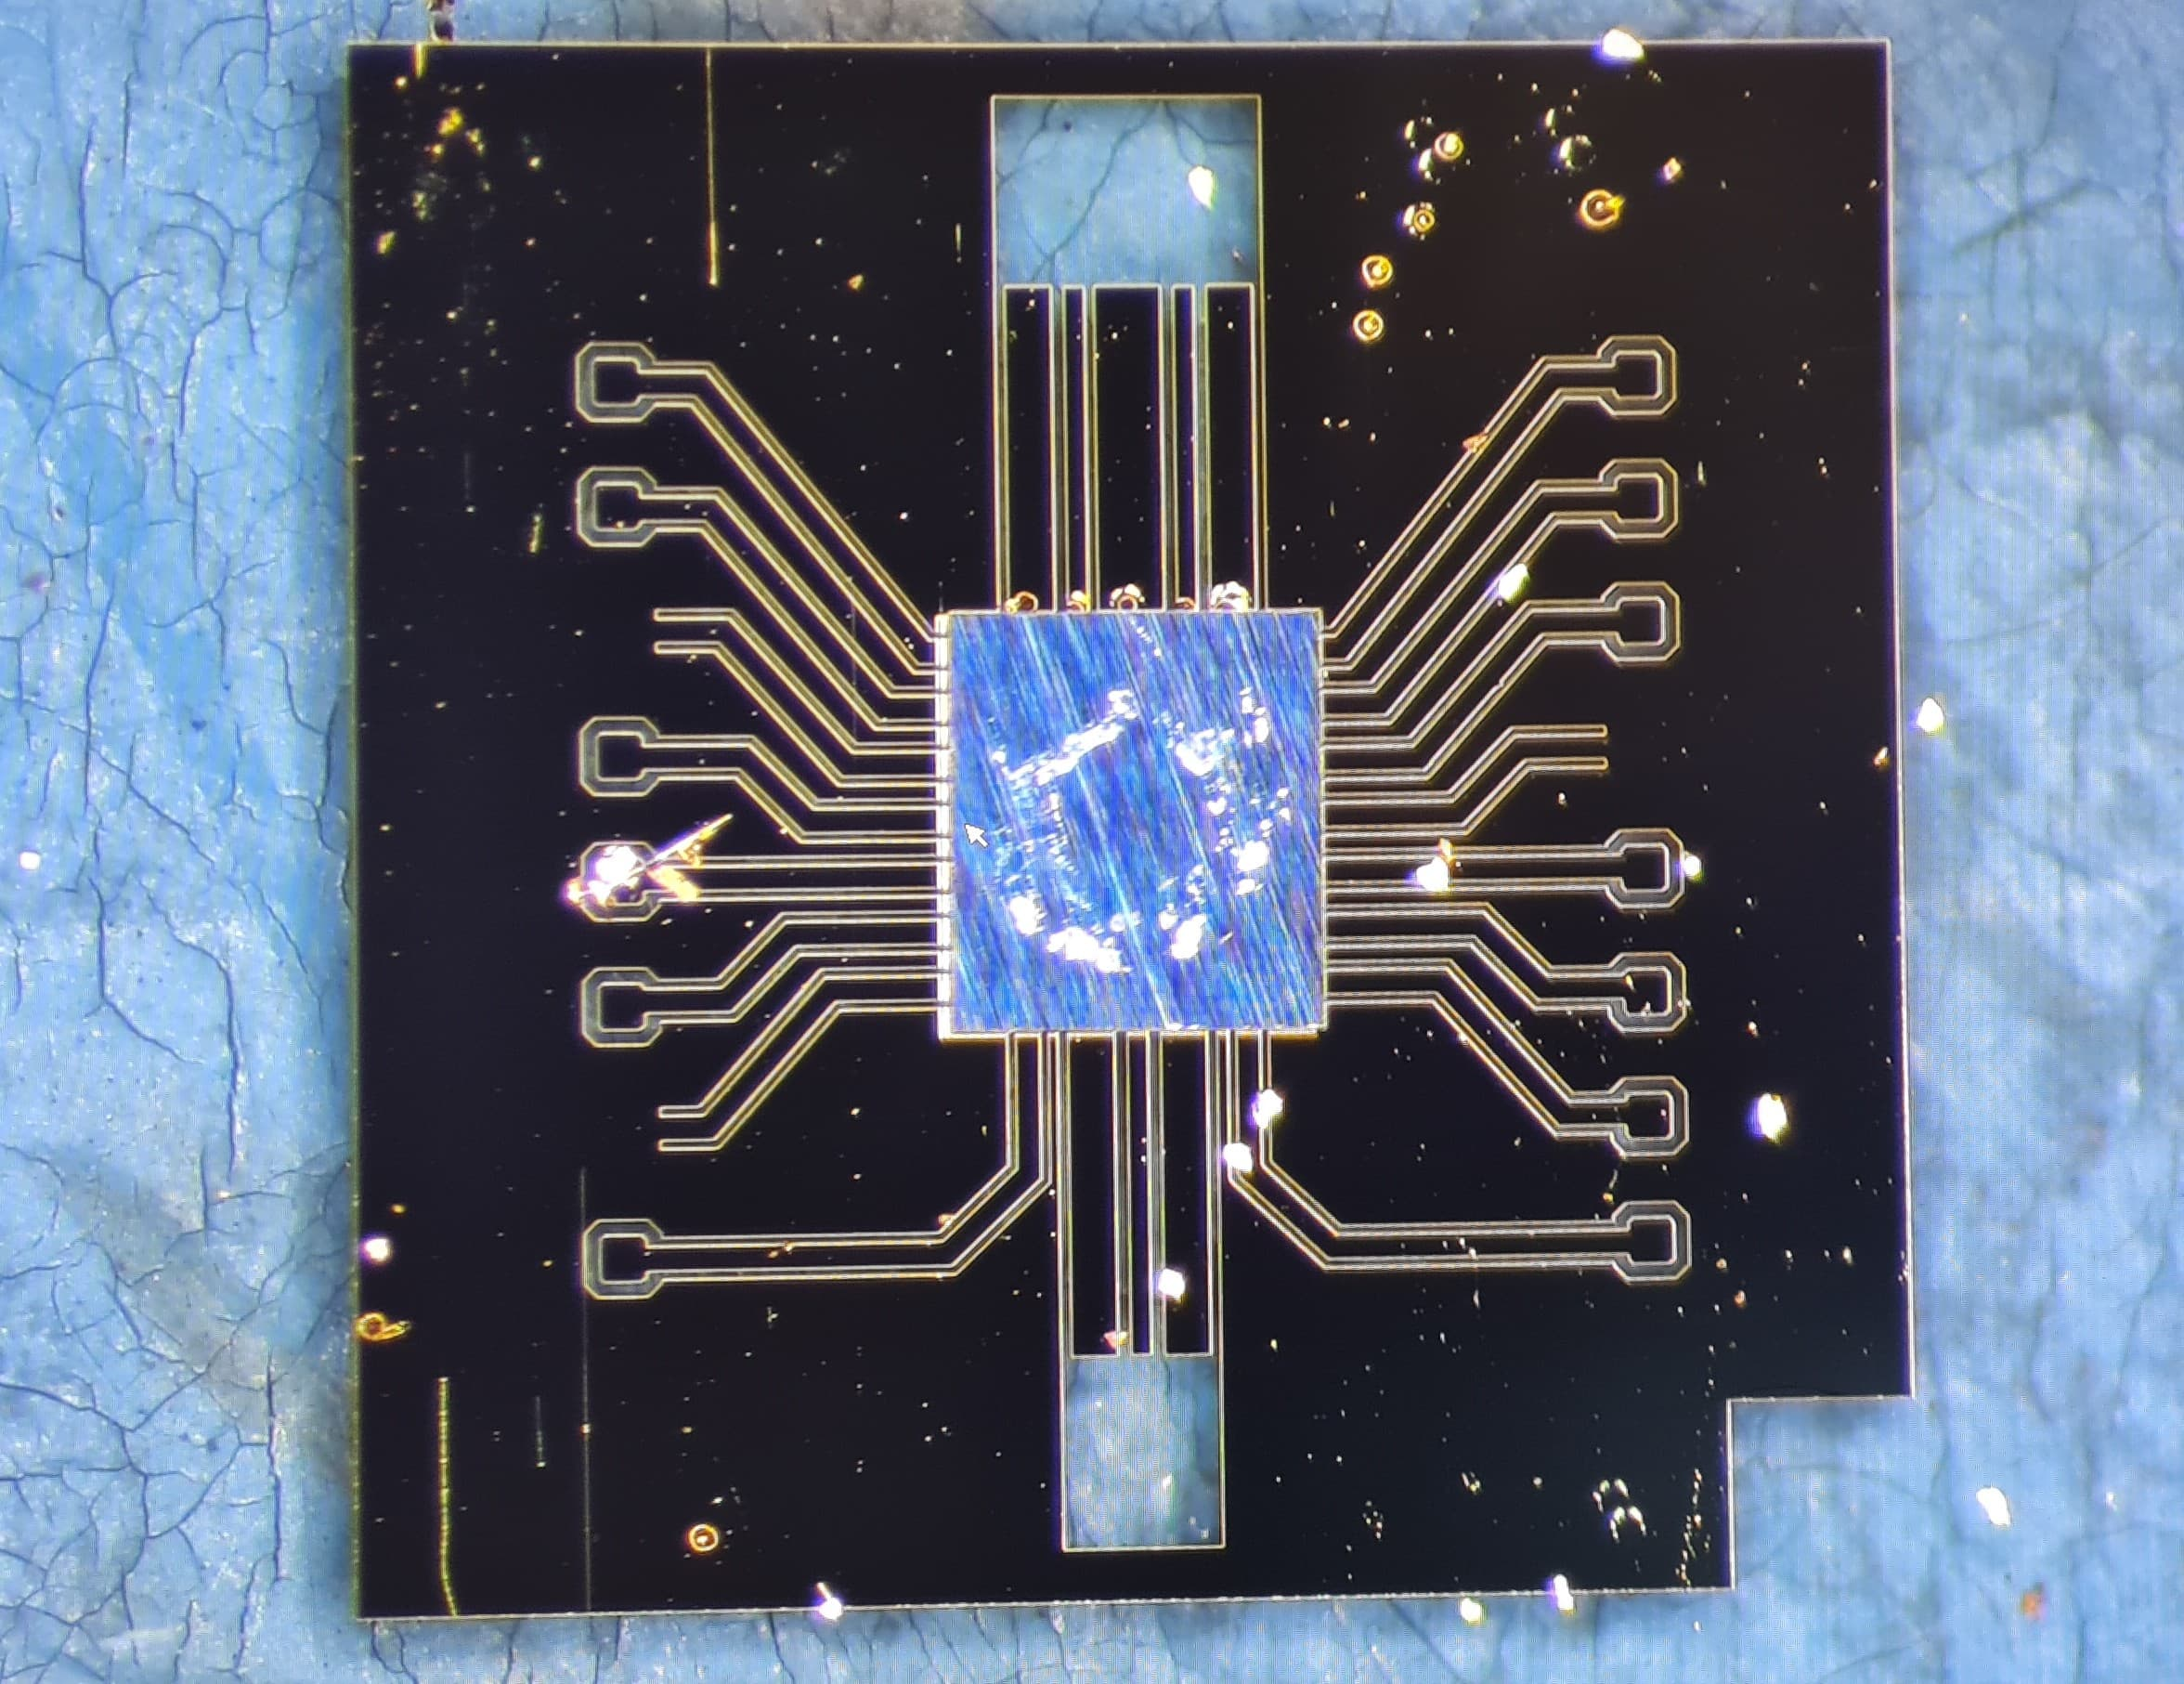
\includegraphics[width=\linewidth]{figures/flip_chipped_die.jpeg}\\[-0.4em]
    (a)
  \end{minipage}\hfill
  \begin{minipage}[t]{0.49\linewidth}
    \centering
    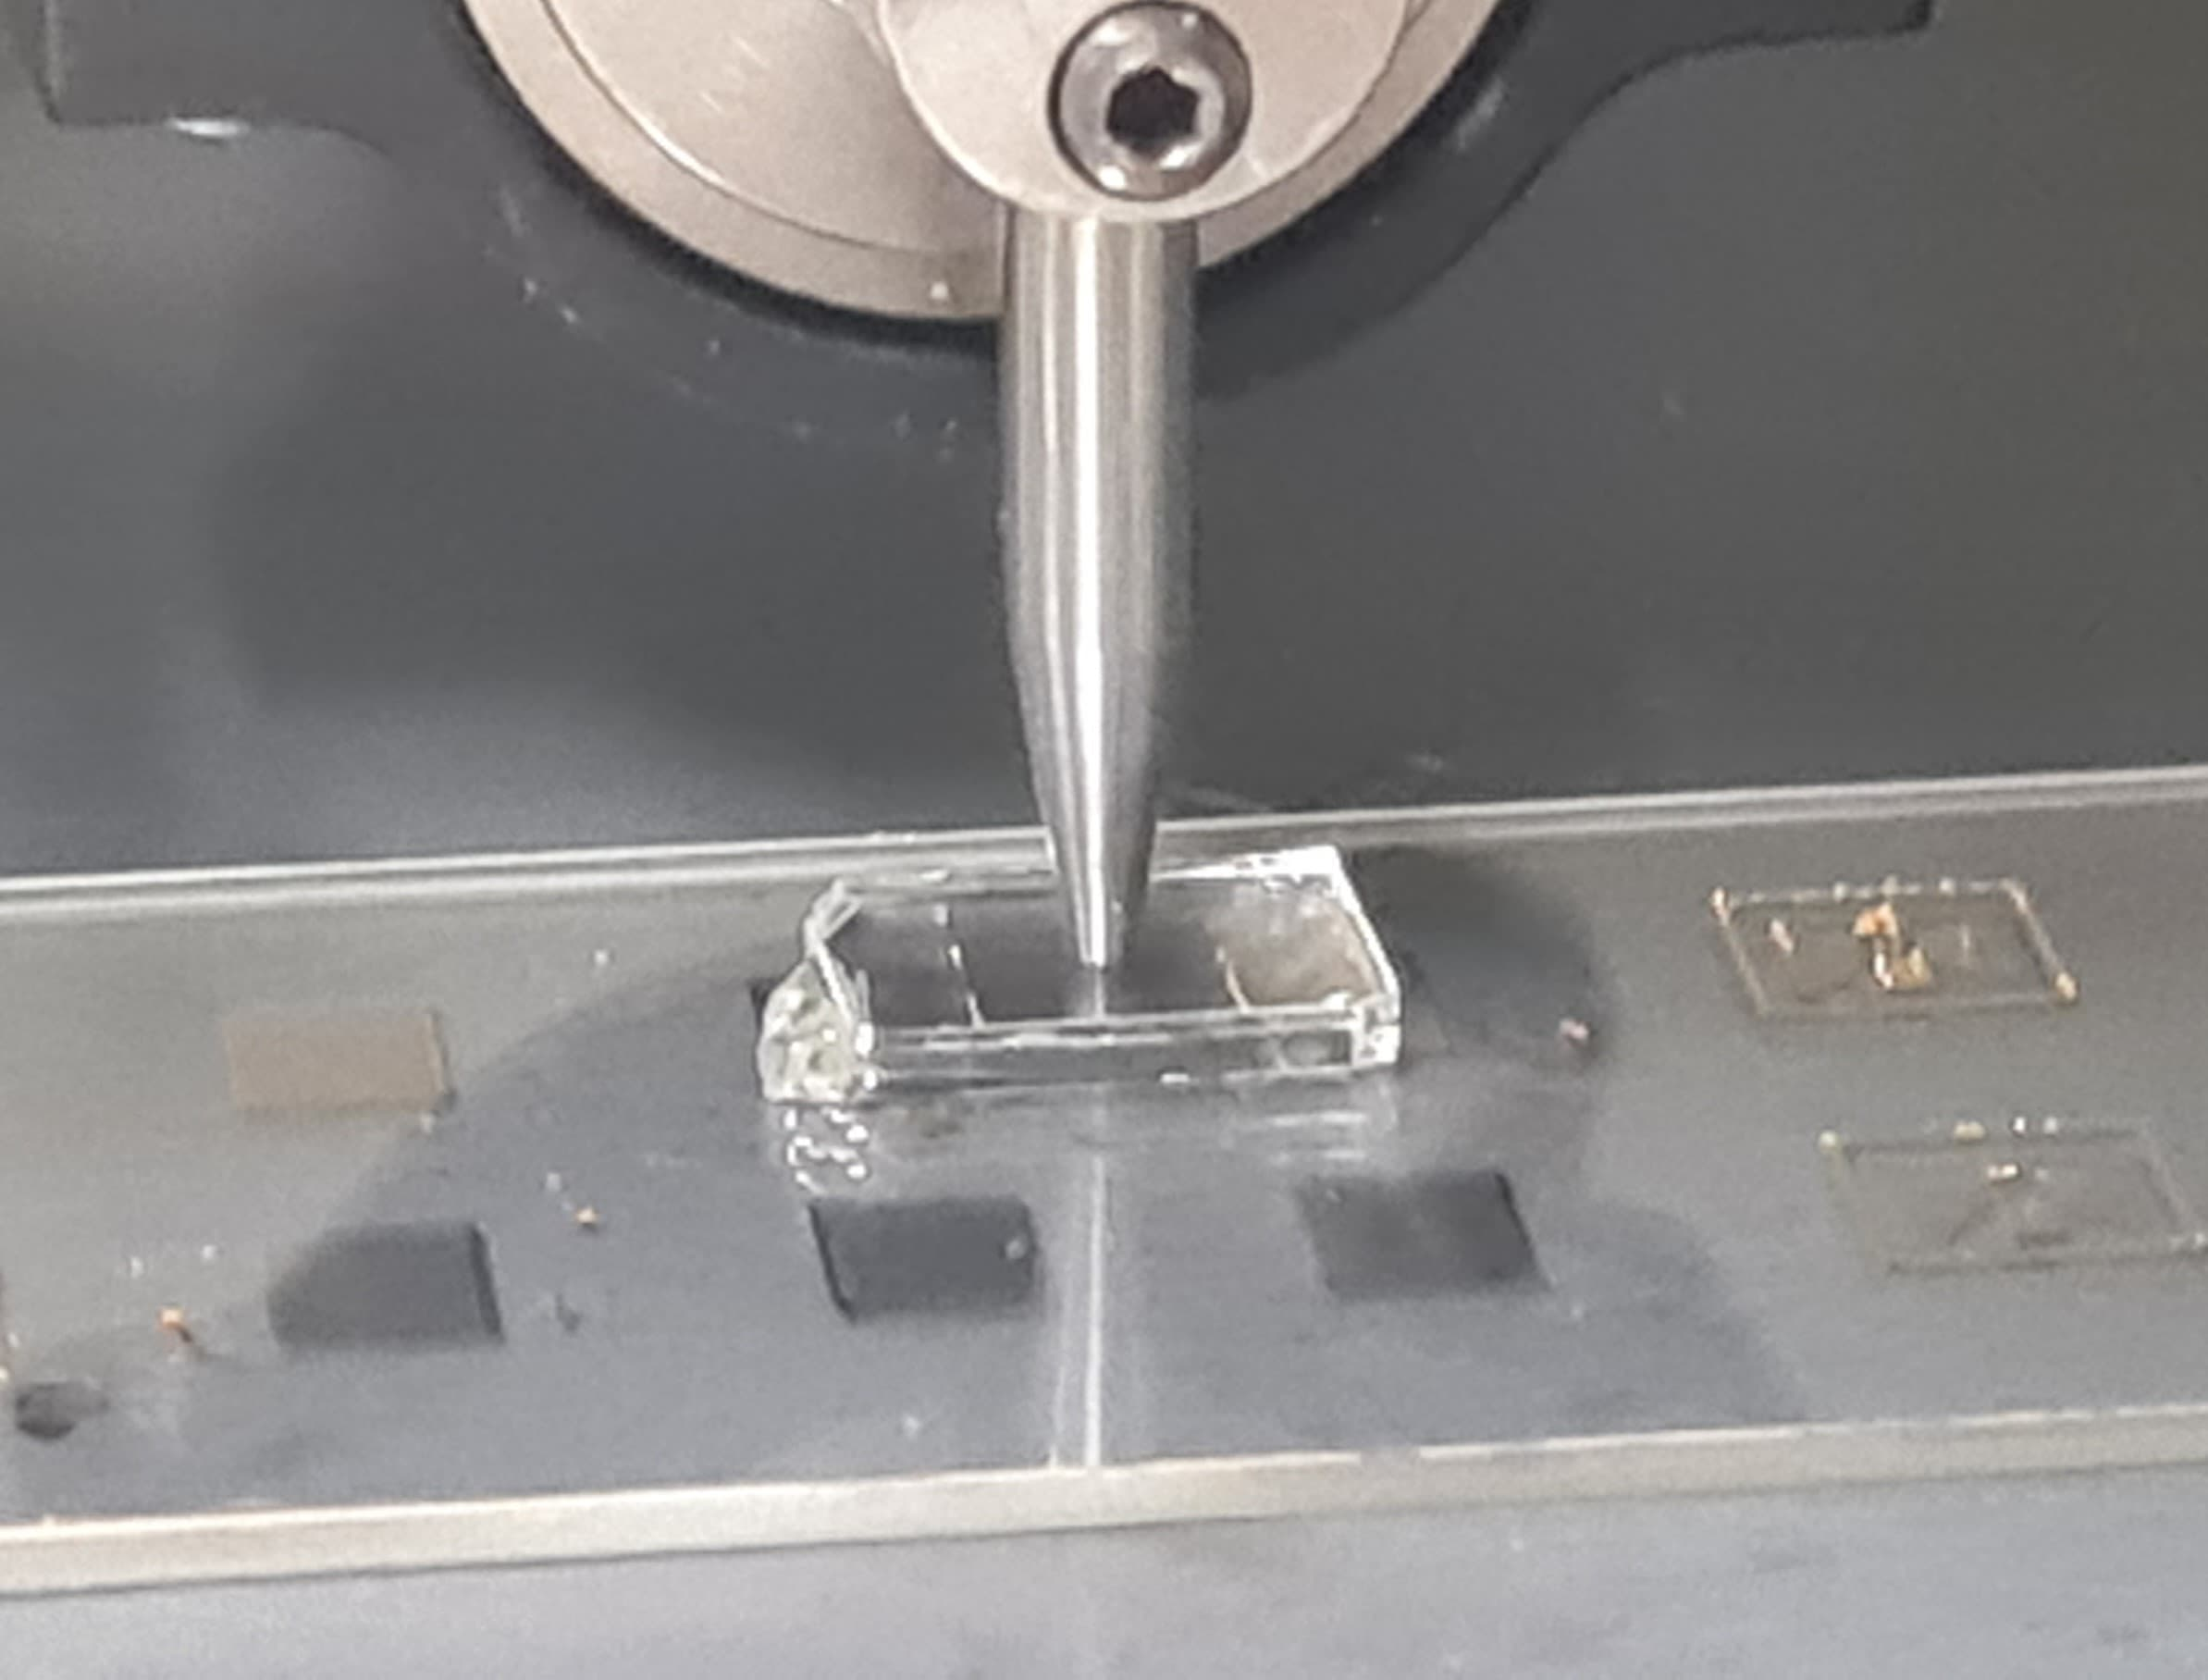
\includegraphics[width=\linewidth]{figures/flip_chipping_fake_die.jpeg}\\[-0.4em]
    (b)
  \end{minipage}
  \caption{Dr.~Tretsky T-5300 bonding:
  (a) fully aligned GaN die (blue square in the middle is the back of the die) flip-chipped onto glass interposer,
  (b) load application during yield-interposer trials at \SI{20}{g}/bump.}
  \label{fig:flipchip_photos}
  \vspace{-10px}
\end{figure}

\subsection{VNA Test Infrastructure}\label{subsec:vna}

All S-parameter measurements were taken on an MPI THz-Selection
probe station fitted with \(\lvert Z\rvert\) GSG probes and a Keysight PNA-X N5247B
(\SI{10}{\mega\hertz}–\SI{10}{\giga\hertz}) seen in Fig.~\ref{fig:vna_setup}. An open-short calibration was performed so that the reference plane coincides with the ends of the CPWG pads.

\begin{figure}[htbp]
  \centering
  \begin{minipage}[t]{0.32\linewidth}
    \centering
    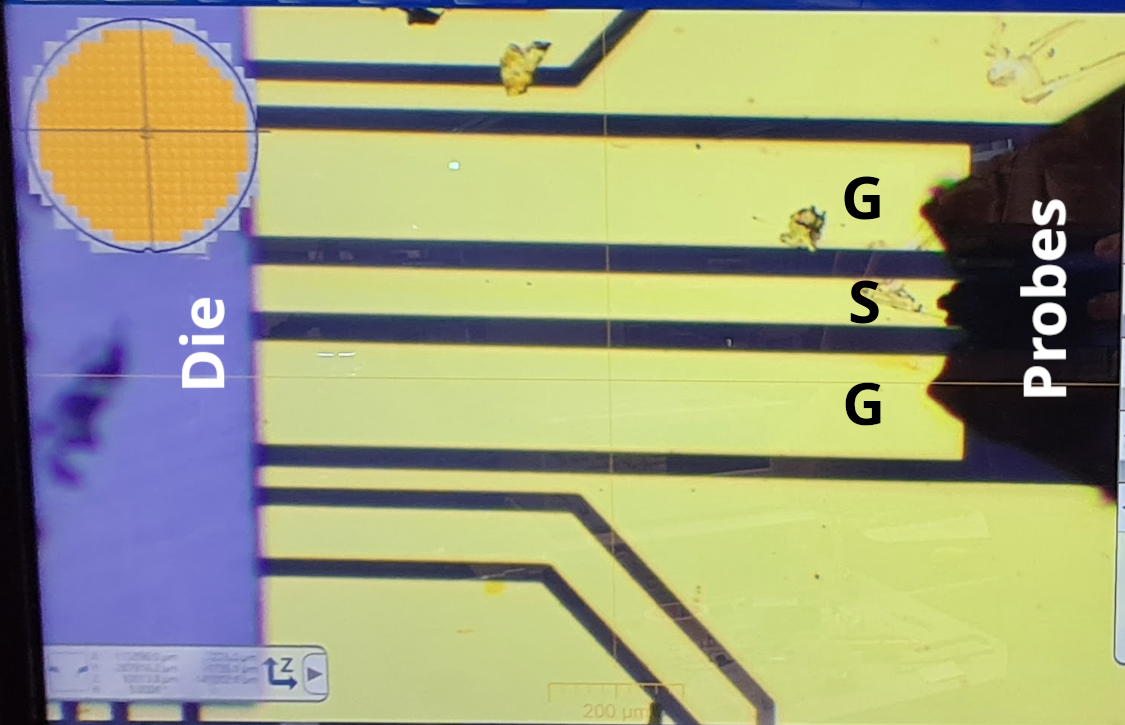
\includegraphics[width=\linewidth]{figures/gsg_probes_labeled.png}\\[-0.4em]
    (a)
  \end{minipage}\hfill
  \begin{minipage}[t]{0.32\linewidth}
    \centering
    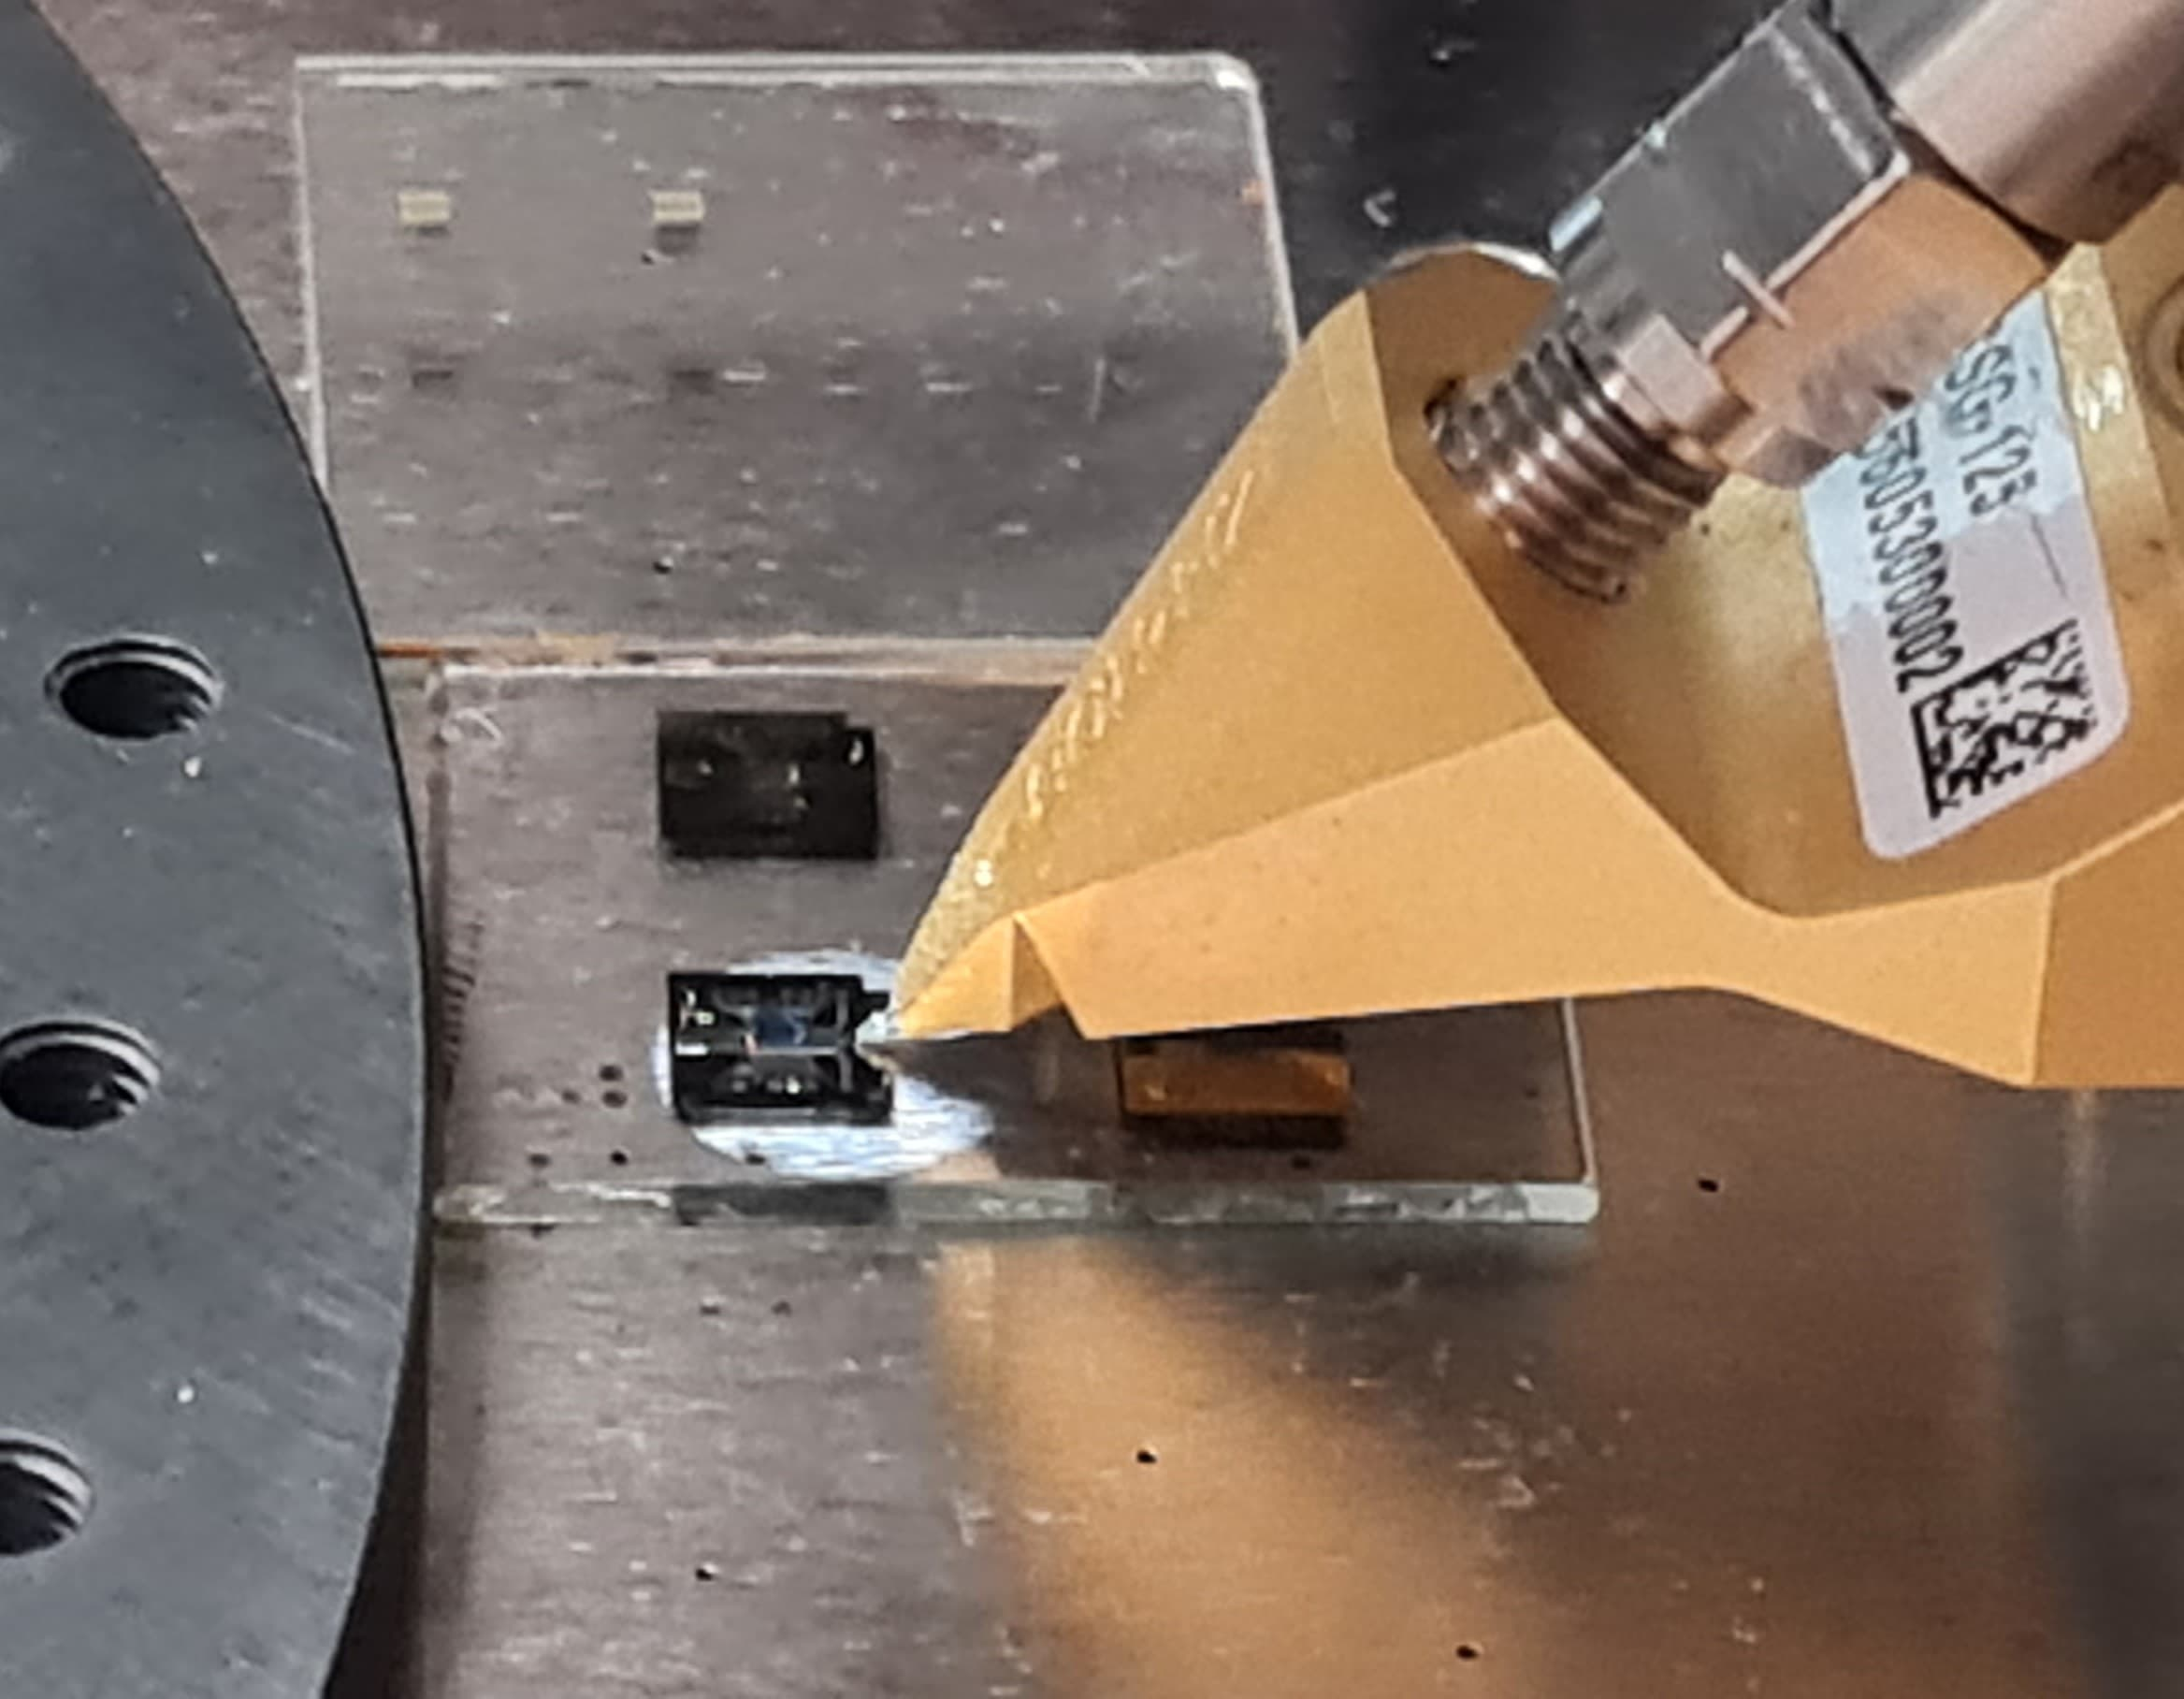
\includegraphics[width=\linewidth]{figures/interposer_probed.jpeg}\\[-0.4em]
    (b)
  \end{minipage}\hfill
  \begin{minipage}[t]{0.32\linewidth}
    \centering
    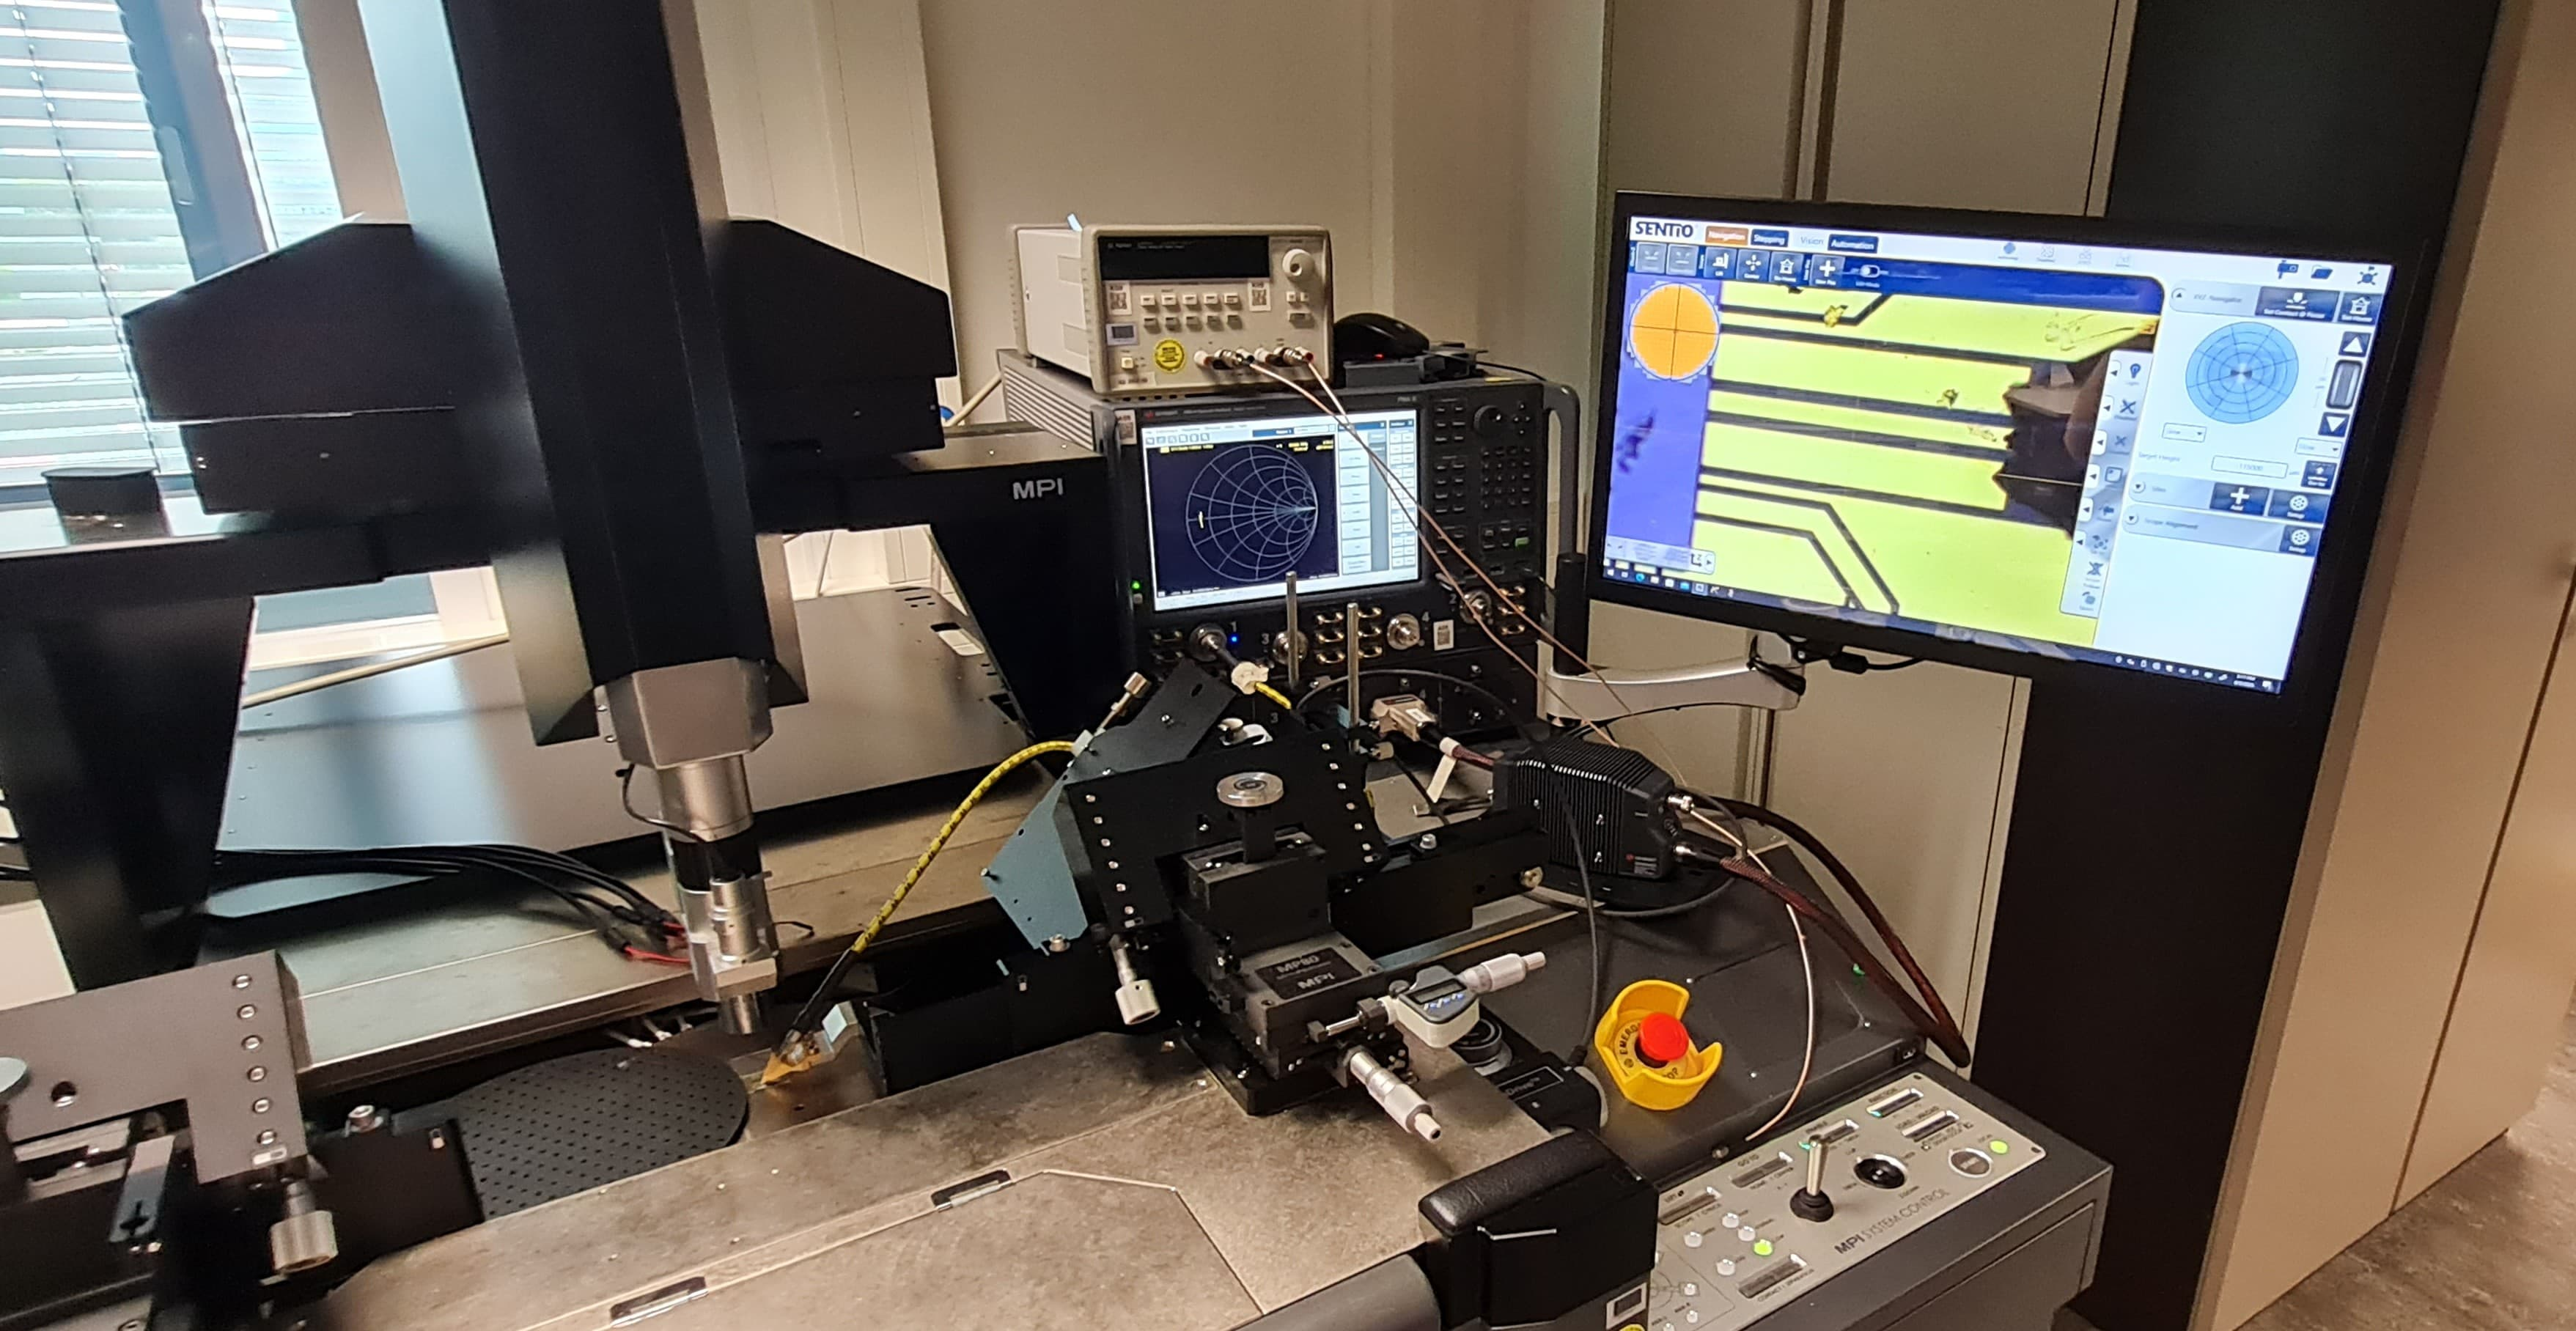
\includegraphics[width=\linewidth]{figures/VNA_machine_setup.jpeg}\\[-0.4em]
    (c)
  \end{minipage}
  \caption{VNA measurement setup:
  (a) microscope view of the \(\lvert Z\rvert\) probe on the GSG pad,
  (b) macro view of the interposer under test,
  (c) Keysight PNA-X connected to the MPI probe station.}
  \label{fig:vna_setup}
    \vspace{-10px}
\end{figure}

\section{Results and Discussion}\label{sec:results}

\subsection{Bump S-Parameters and De-embedding (10 MHz–10 GHz)}
\label{subsec:bump_deemb}

The de-embedding follows the improved open–short method
of \cite{Konstantinou2021}.  
Three impedances are measured: OPEN, SHORT, and DUT, the
latter comprising the TXFE die, three Au bumps, and the
\SI{1.15}{mm} GSG trace Fig.~\ref{fig:deembed_schem}. The impedance is obtained from
%
\begin{equation}
Z(f)=Z_{0}\,\frac{1+S_{11}(f)}{1-S_{11}(f)},
\label{eq:z_raw}
\end{equation}
%
and the trace is removed via the improved open-short equation,
%
\begin{equation}
Z_{\!\text{de}}(f)=Z_{\text{OC}}(f)\,
\frac{Z_{m}(f)-Z_{\text{SC}}(f)}{Z_{\text{OC}}(f)-Z_{m}(f)}.
\label{eq:z_de}
\end{equation}
%
Subtracting the die input impedance isolates the three-bump transition
and scaling by \(2/3\) yields a single bump:
%
\begin{equation}
Z_{b}(f)=\tfrac{2}{3}\bigl[Z_{\!\text{de}}(f)-Z_{\text{die}}(f)\bigr].
\label{eq:z_bump}
\end{equation}

\medskip
Fig.~\ref{fig:deembed_magphase} overlays the magnitude and phase of
$S_{11}$. The curve labeled DUT represents the full
die+3-bump+trace system, while the curve labeled "De-embedded"
is obtained after changing the reference plane with \eqref{eq:z_de}.
All parameters are evaluated with the lowest frequency
(\SI{10}{MHz}) to minimize residual parasitics from the pads and probes. At that point \(R_{\text{bump}}=\SI{3.4}{\ohm}\) is obtained, three orders of magnitude above the \SI{0.24}{\milli\ohm} predicted for 3 bumps in section \ref{subsec:bump_line_model}.  
The divergence is attributed to gaps or oxides at the Au–Au interface
and spreading resistance in the pads, phenomena that are absent from the closed-form model.

\begin{figure}[htbp]
  \centering
  \begin{minipage}[t]{0.49\linewidth}
    \centering
    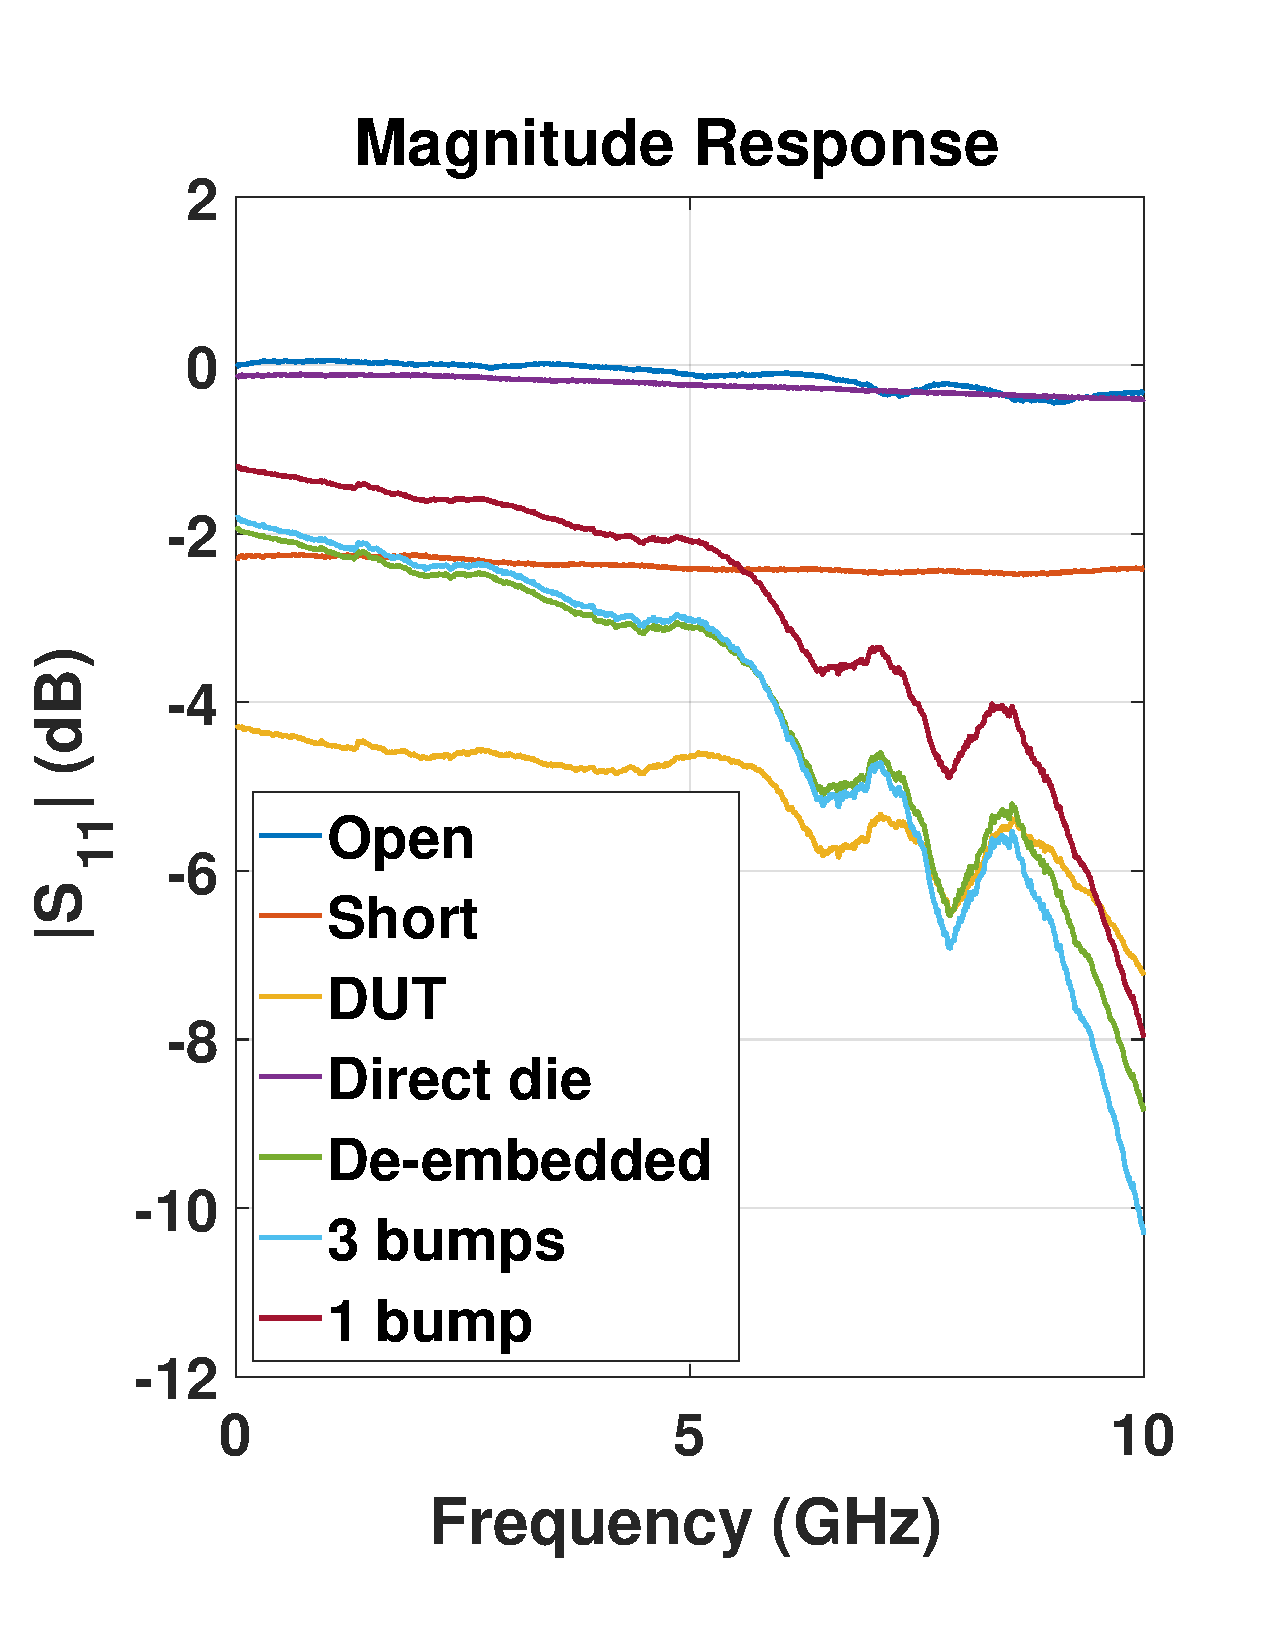
\includegraphics[width=\linewidth]{figures/magnitude_final.pdf}\\[-0.3em]
    (a)
  \end{minipage}\hfill
  \begin{minipage}[t]{0.49\linewidth}
    \centering
    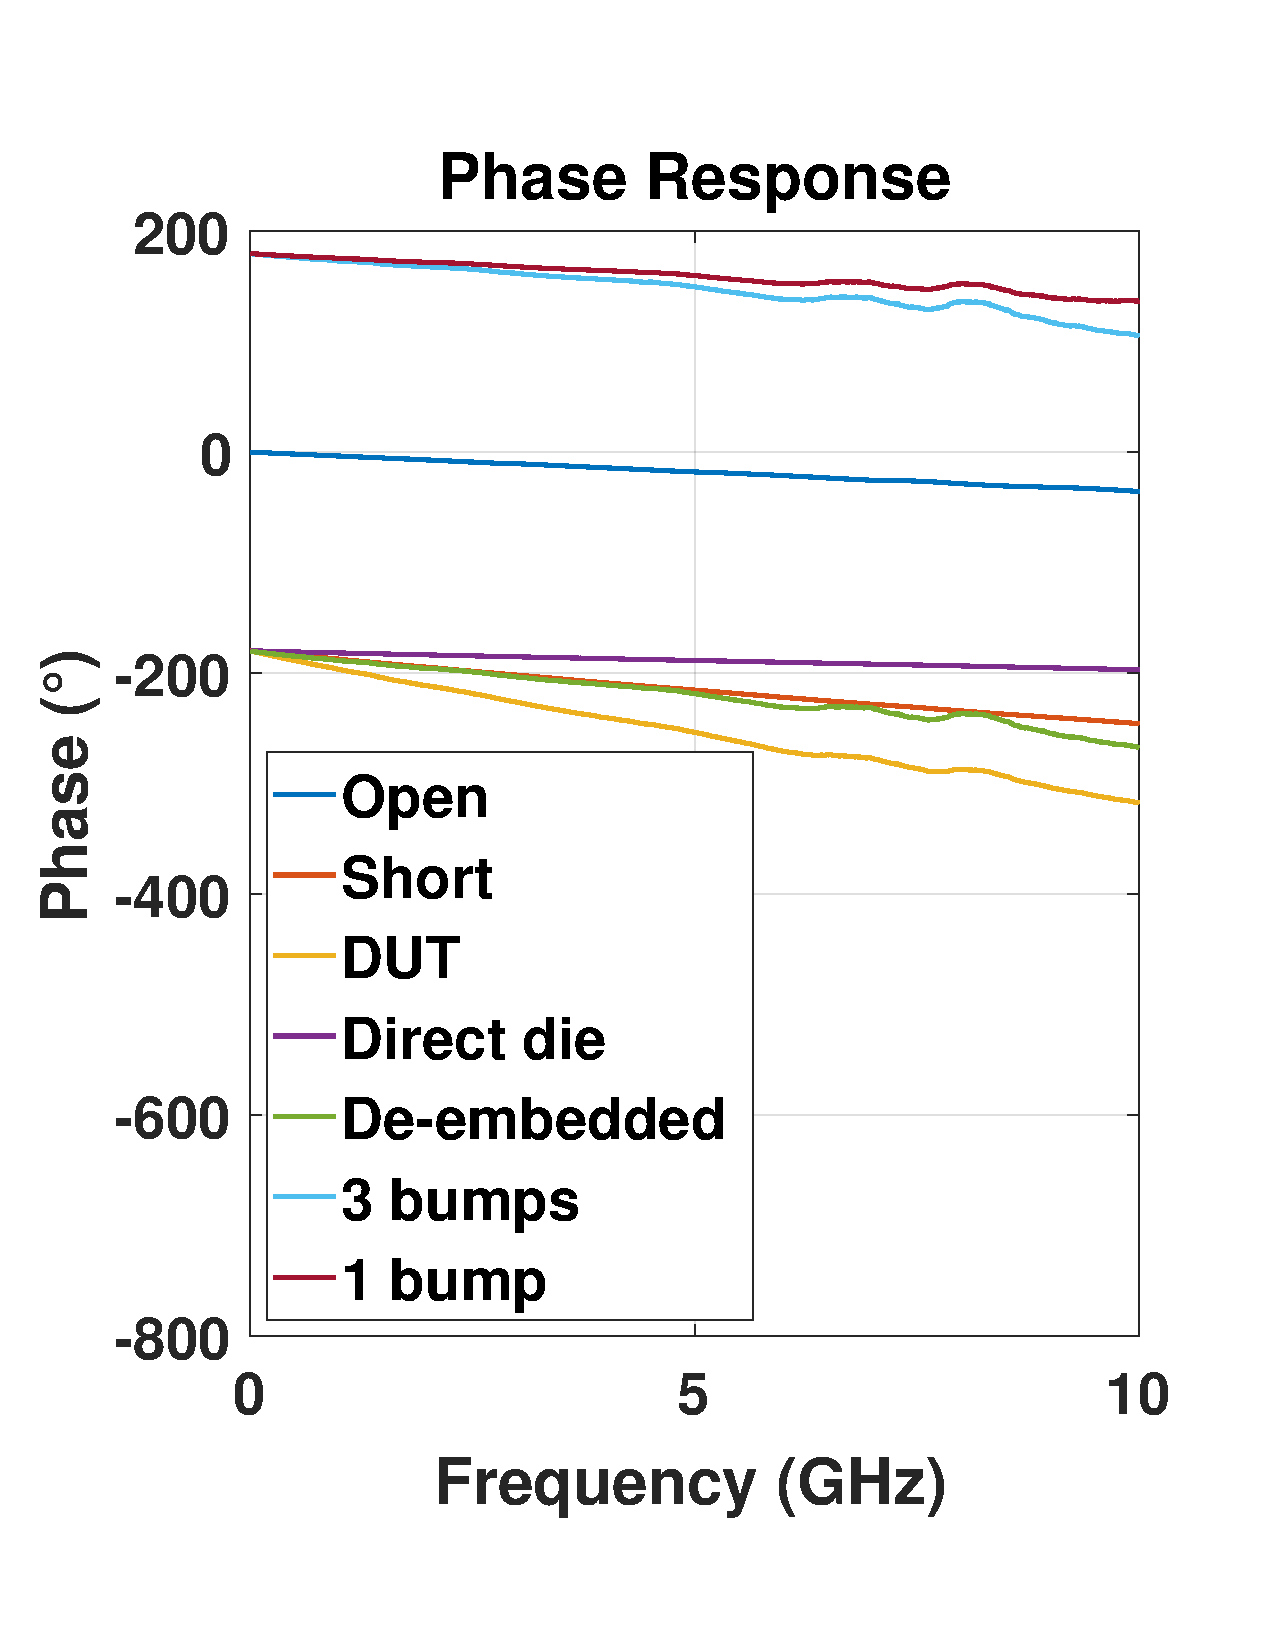
\includegraphics[width=\linewidth]{figures/phase_finalist.pdf}\\[-0.3em]
    (b)
  \end{minipage}
  \caption{$S_{11}$ magnitude and phase before and after
  de-embedding.  The DUT trace refers to the raw
  die+3-bump+trace measurement, while "De-embedded" refers to the
  response after reference-plane shift.}
  \label{fig:deembed_magphase}
  \vspace{-10px}
\end{figure}

\begin{figure}[htbp]
  \centering
  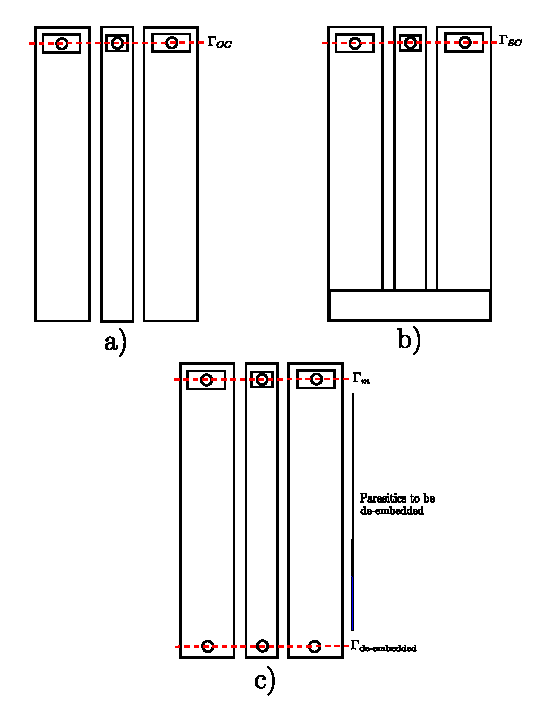
\includegraphics[angle=-90,width=\linewidth]{figures/deembedding.pdf}
  \caption{Open (a), short (b) and DUT (c) calibration structures indicating the reference-plane shift (dashed red line).}
  \label{fig:deembed_schem}
  \vspace{-10pt}
\end{figure}

\begin{figure}[htbp]
  \centering
  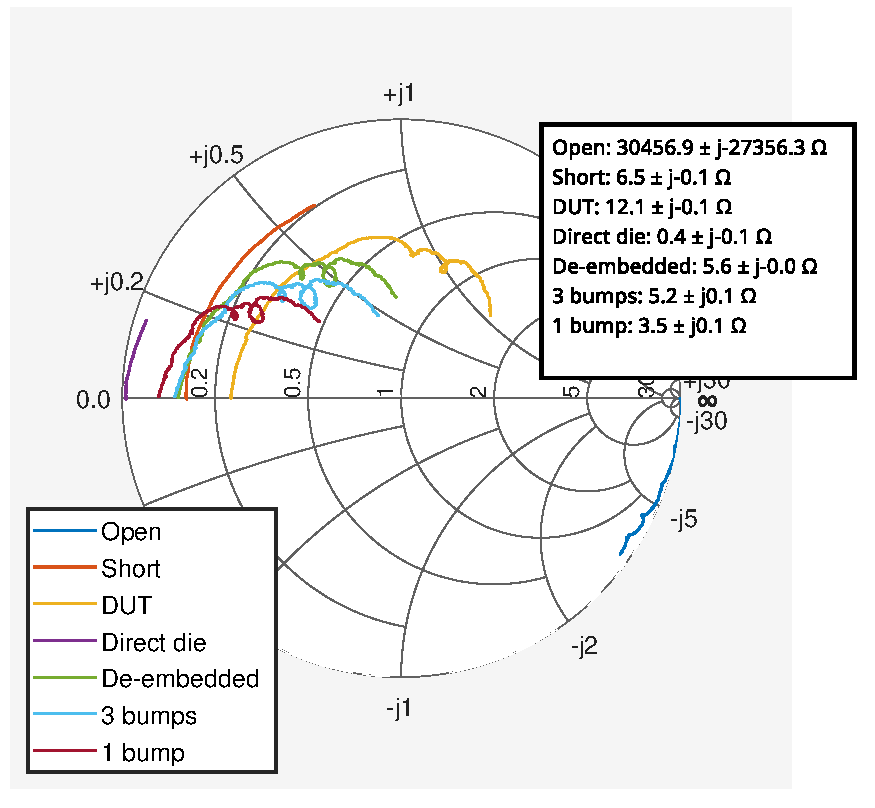
\includegraphics[width=\linewidth]{figures/deembedding_smithchart.pdf}
  \caption{Smith chart of $S_{11}$ through the de-embedding sequence.}
  \label{fig:deembed_smithchart}
  \vspace{-10pt}
\end{figure}


\subsection{CPWG Line RLCG and Bump RLC Parameters}
\label{subsec:rlcg}

The lumped parameters of the GSG trace \SI{1.15}{mm} were extracted from
the OPEN–SHORT data using the procedure of
\cite{Eisenstadt1992}. Scaling by $10^{-6}$ converts $R',L',C',G'$ to the \si{\micro\metre}
basis used in section \ref{subsec:bump_line_model}.  
Fig.~\ref{fig:rlcg_gsg} plots the measured $RLCG$ values; at sub \SI{}{\giga\hertz} the line gives around $R=\SI{5.4}{\ohm}$, $L=\SI{0.50}{\nano\henry}$, $C=\SI{65}{\femto\farad}$ within \SI{3}{\percent} of the simulated targets, confirming the validity of the single–metal CPWG model.

The bump impedance was obtained from \eqref{eq:z_bump}.  The real and imaginary parts were converted to $R$, $L_{\text{eq}}=\Im\{Z\}/\omega$
and $C_{\text{eq}}=-1/(\omega\,\Im\{Z\})$; results are shown in
Fig.~\ref{fig:rlc_bump}. At sub \SI{}{\giga\hertz} one stud exhibits
$R_{\text{bump}}=\SI{3.46}{\ohm}$ Fig.~\ref{fig:deembed_smithchart} three decades above the
\SI{0.24}{\milli\ohm} predicted for the ideal 3 bump connection.

Fig.~\ref{fig:sim_real} overlays the simulated $S_{11}$ of
the \textsc{qucs} circuit with the measured $S_{22}$ of the complete
die + 3-bump + GSG structure. In the smith chart the experimental trajectory migrates toward the
center after de-embedding, mirroring the simulated locus.  
Numerically, the simulation predicts $|S_{11}|=\SI{-2.08}{dB}$ at
\SI{10}{MHz}; the raw measurement gives
$|S_{22}|=\SI{-4.30}{dB}$. The mismatch corresponds to
$Z_{22,\text{de}}=\bigl(12.1-j\,0.10\bigr)\,\si{\ohm}$ versus the
ideal \(\sim\!6\,\si{\ohm}\); this offset is consistent with the
resistance to a single bump \SI{3.4}{\ohm} extracted earlier and confirms
that the resistance to bump spreading, not CPWG parasitics, sets the practical
return-loss floor.

DC resistivity and sheet resistance verification. A ground trace was biased in DC to validate the RF extracted
$\rho$ and $R_{\square}$.  With
$R_{\text{DC}}=\SI{2.5}{\ohm}$ for a
$L=\SI{1.15}{mm}$, $W=\SI{153}{\micro\metre}$,
$t=\SI{150}{\nano\metre}$ section,
%
\begin{equation}
A = Wt = 153\times10^{-6}\!\times150\times10^{-9}
       = 2.295\times10^{-11}\;\text{m}^2,
\label{eq:area}
\end{equation}
%
\begin{equation}
\rho = R_{\text{DC}}\frac{A}{L}
      = 2.5\:\Omega\;
        \frac{2.295\times10^{-11}}{1.15\times10^{-3}}
      = 4.99\times10^{-8}\;\Omega\!\cdot\!\text{m},
\label{eq:rho_calc}
\end{equation}
%
\begin{equation}
R_{\square} = \frac{\rho}{t}
            = \frac{4.99\times10^{-8}}{150\times10^{-9}}
            \approx 0.333\;\Omega/\square .
\label{eq:sheet}
\end{equation}
%
The predictions based on Eq. \eqref{eq:rho_calc}–\eqref{eq:sheet} closely match the results obtained
from the broadband \(RLCG\) fit Fig.~\ref{fig:rlcg_gsg}.

\begin{figure}[htbp]
  \centering
  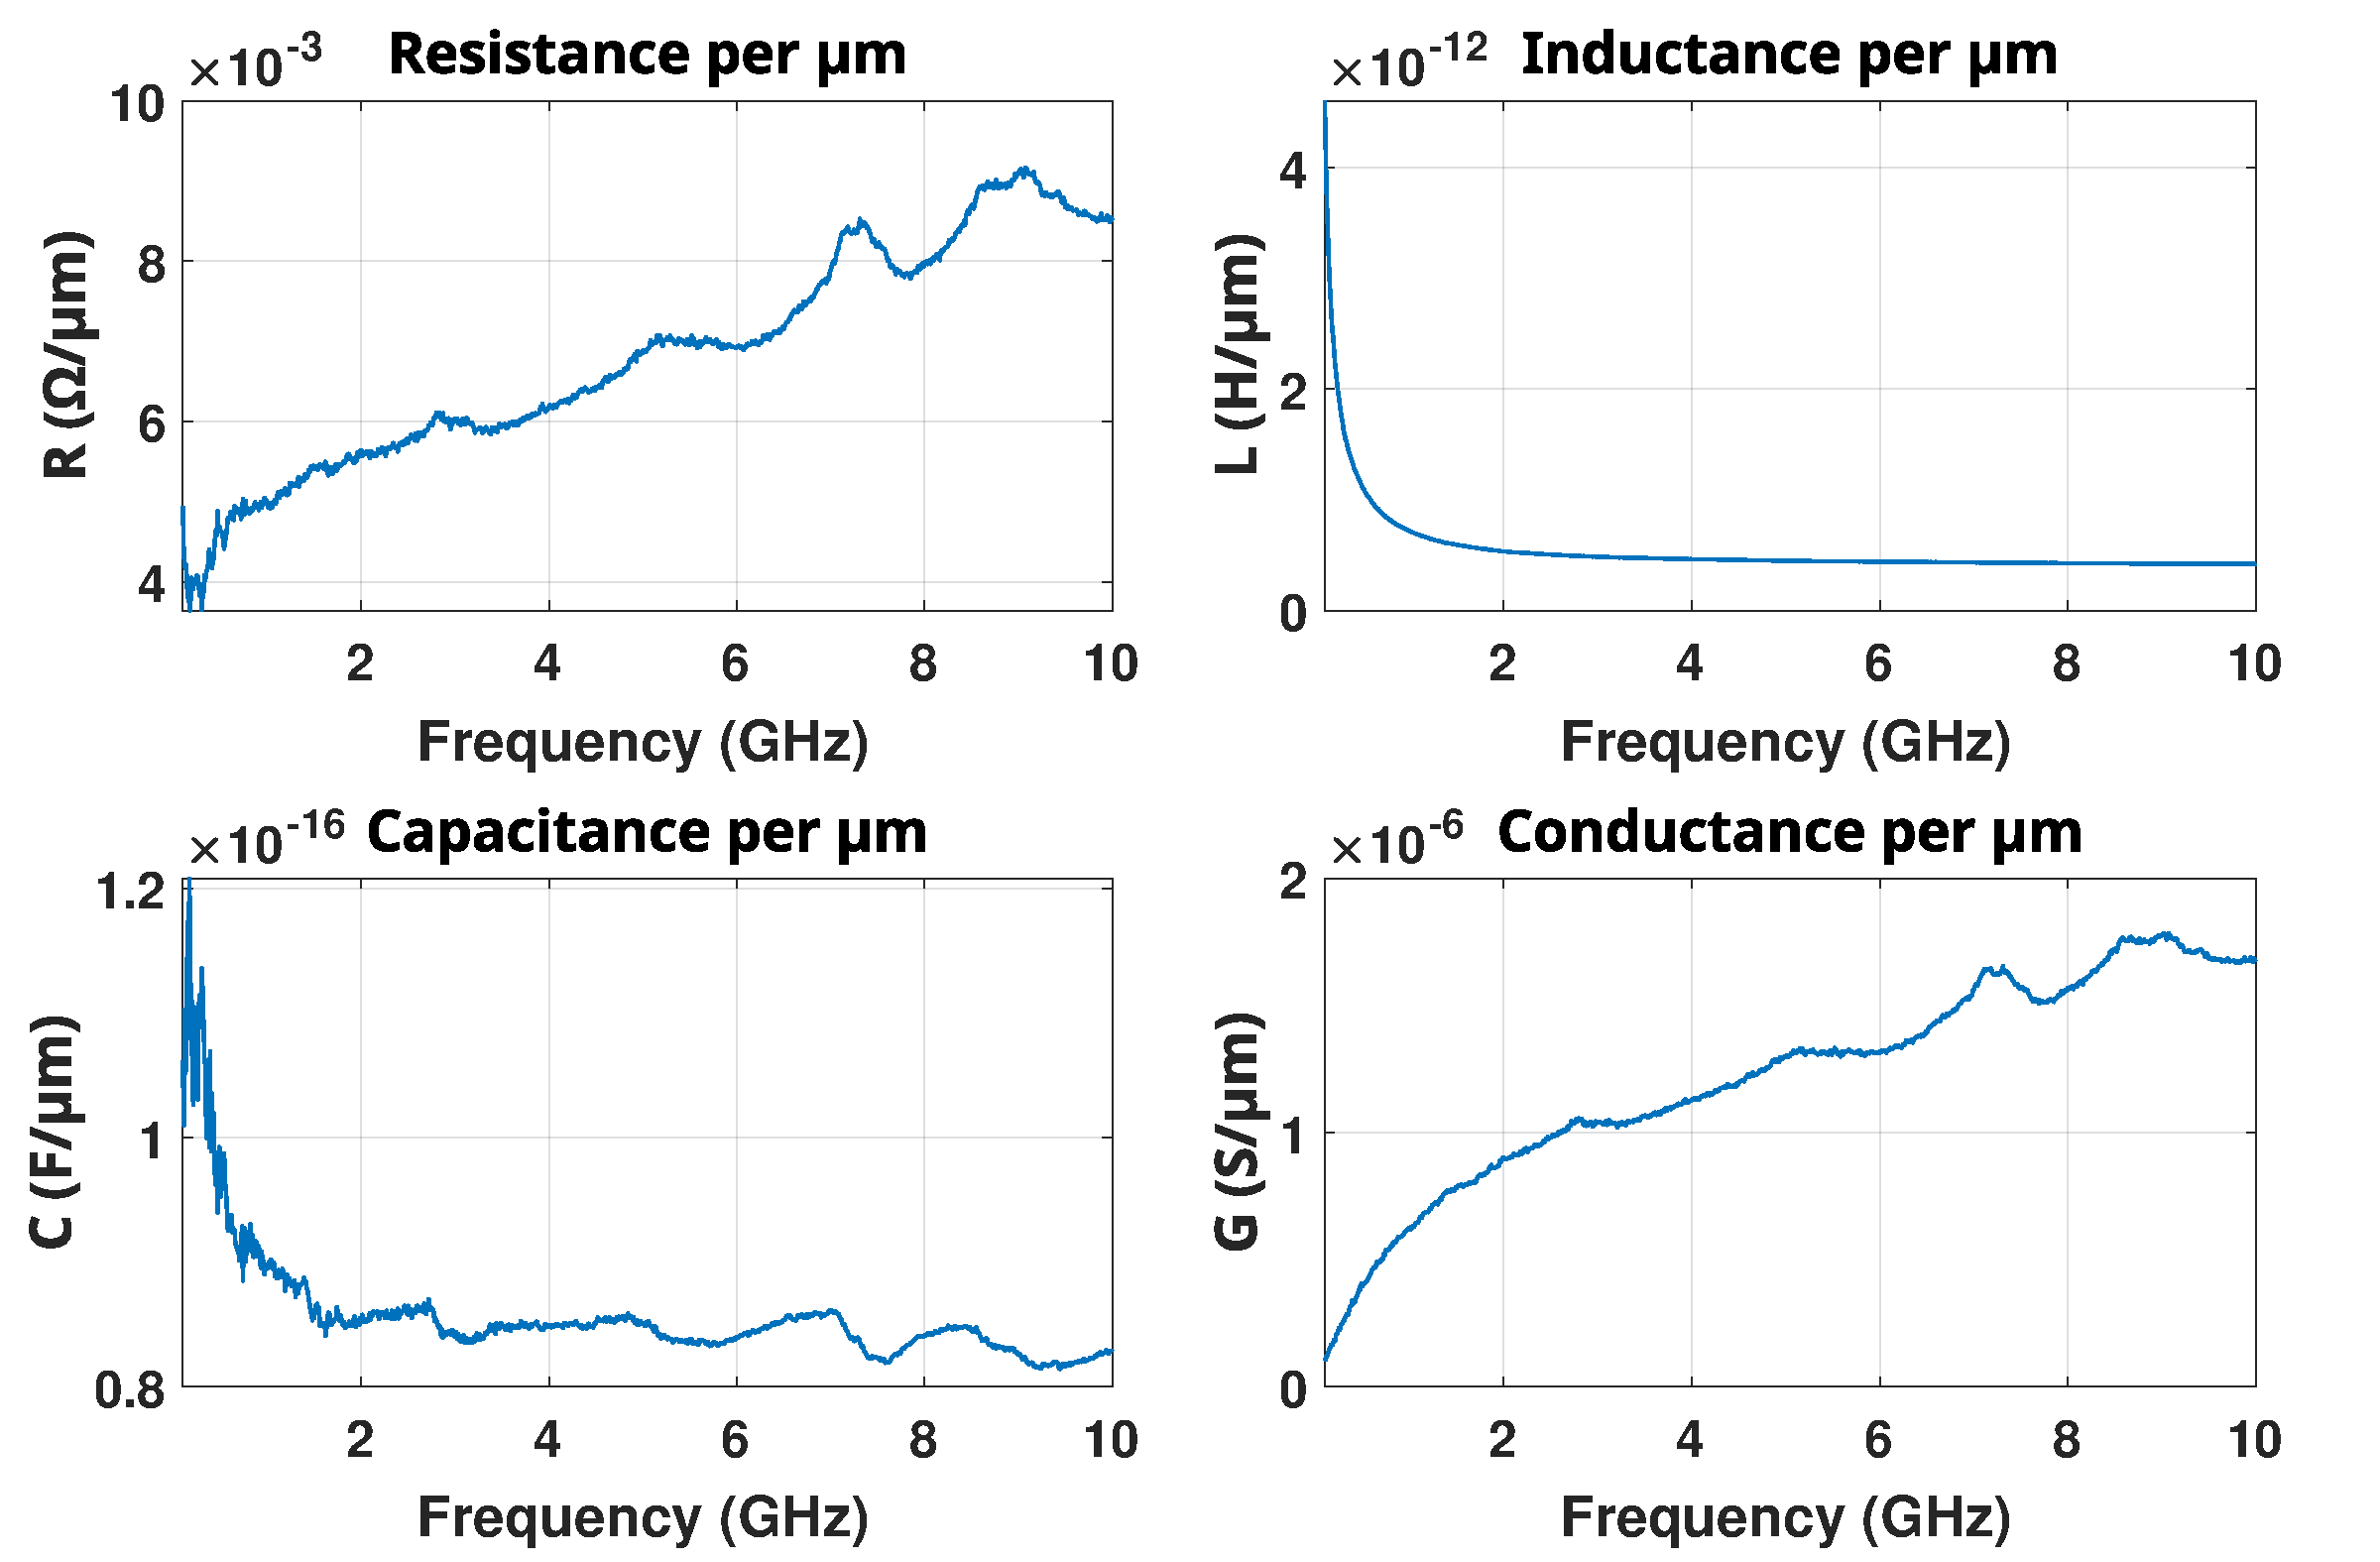
\includegraphics[width=\linewidth]{figures/RLCG_FINAL_FINAL_FINAL.pdf}
  \caption{Extracted RLCG values of a \SI{1.15}{mm} GSG line (\SI{10}{\mega\hertz} - \SI{10}{\giga\hertz}).}
  \label{fig:rlcg_gsg}
  \vspace{-15px}
\end{figure}

\begin{figure}[htbp]
  \centering
  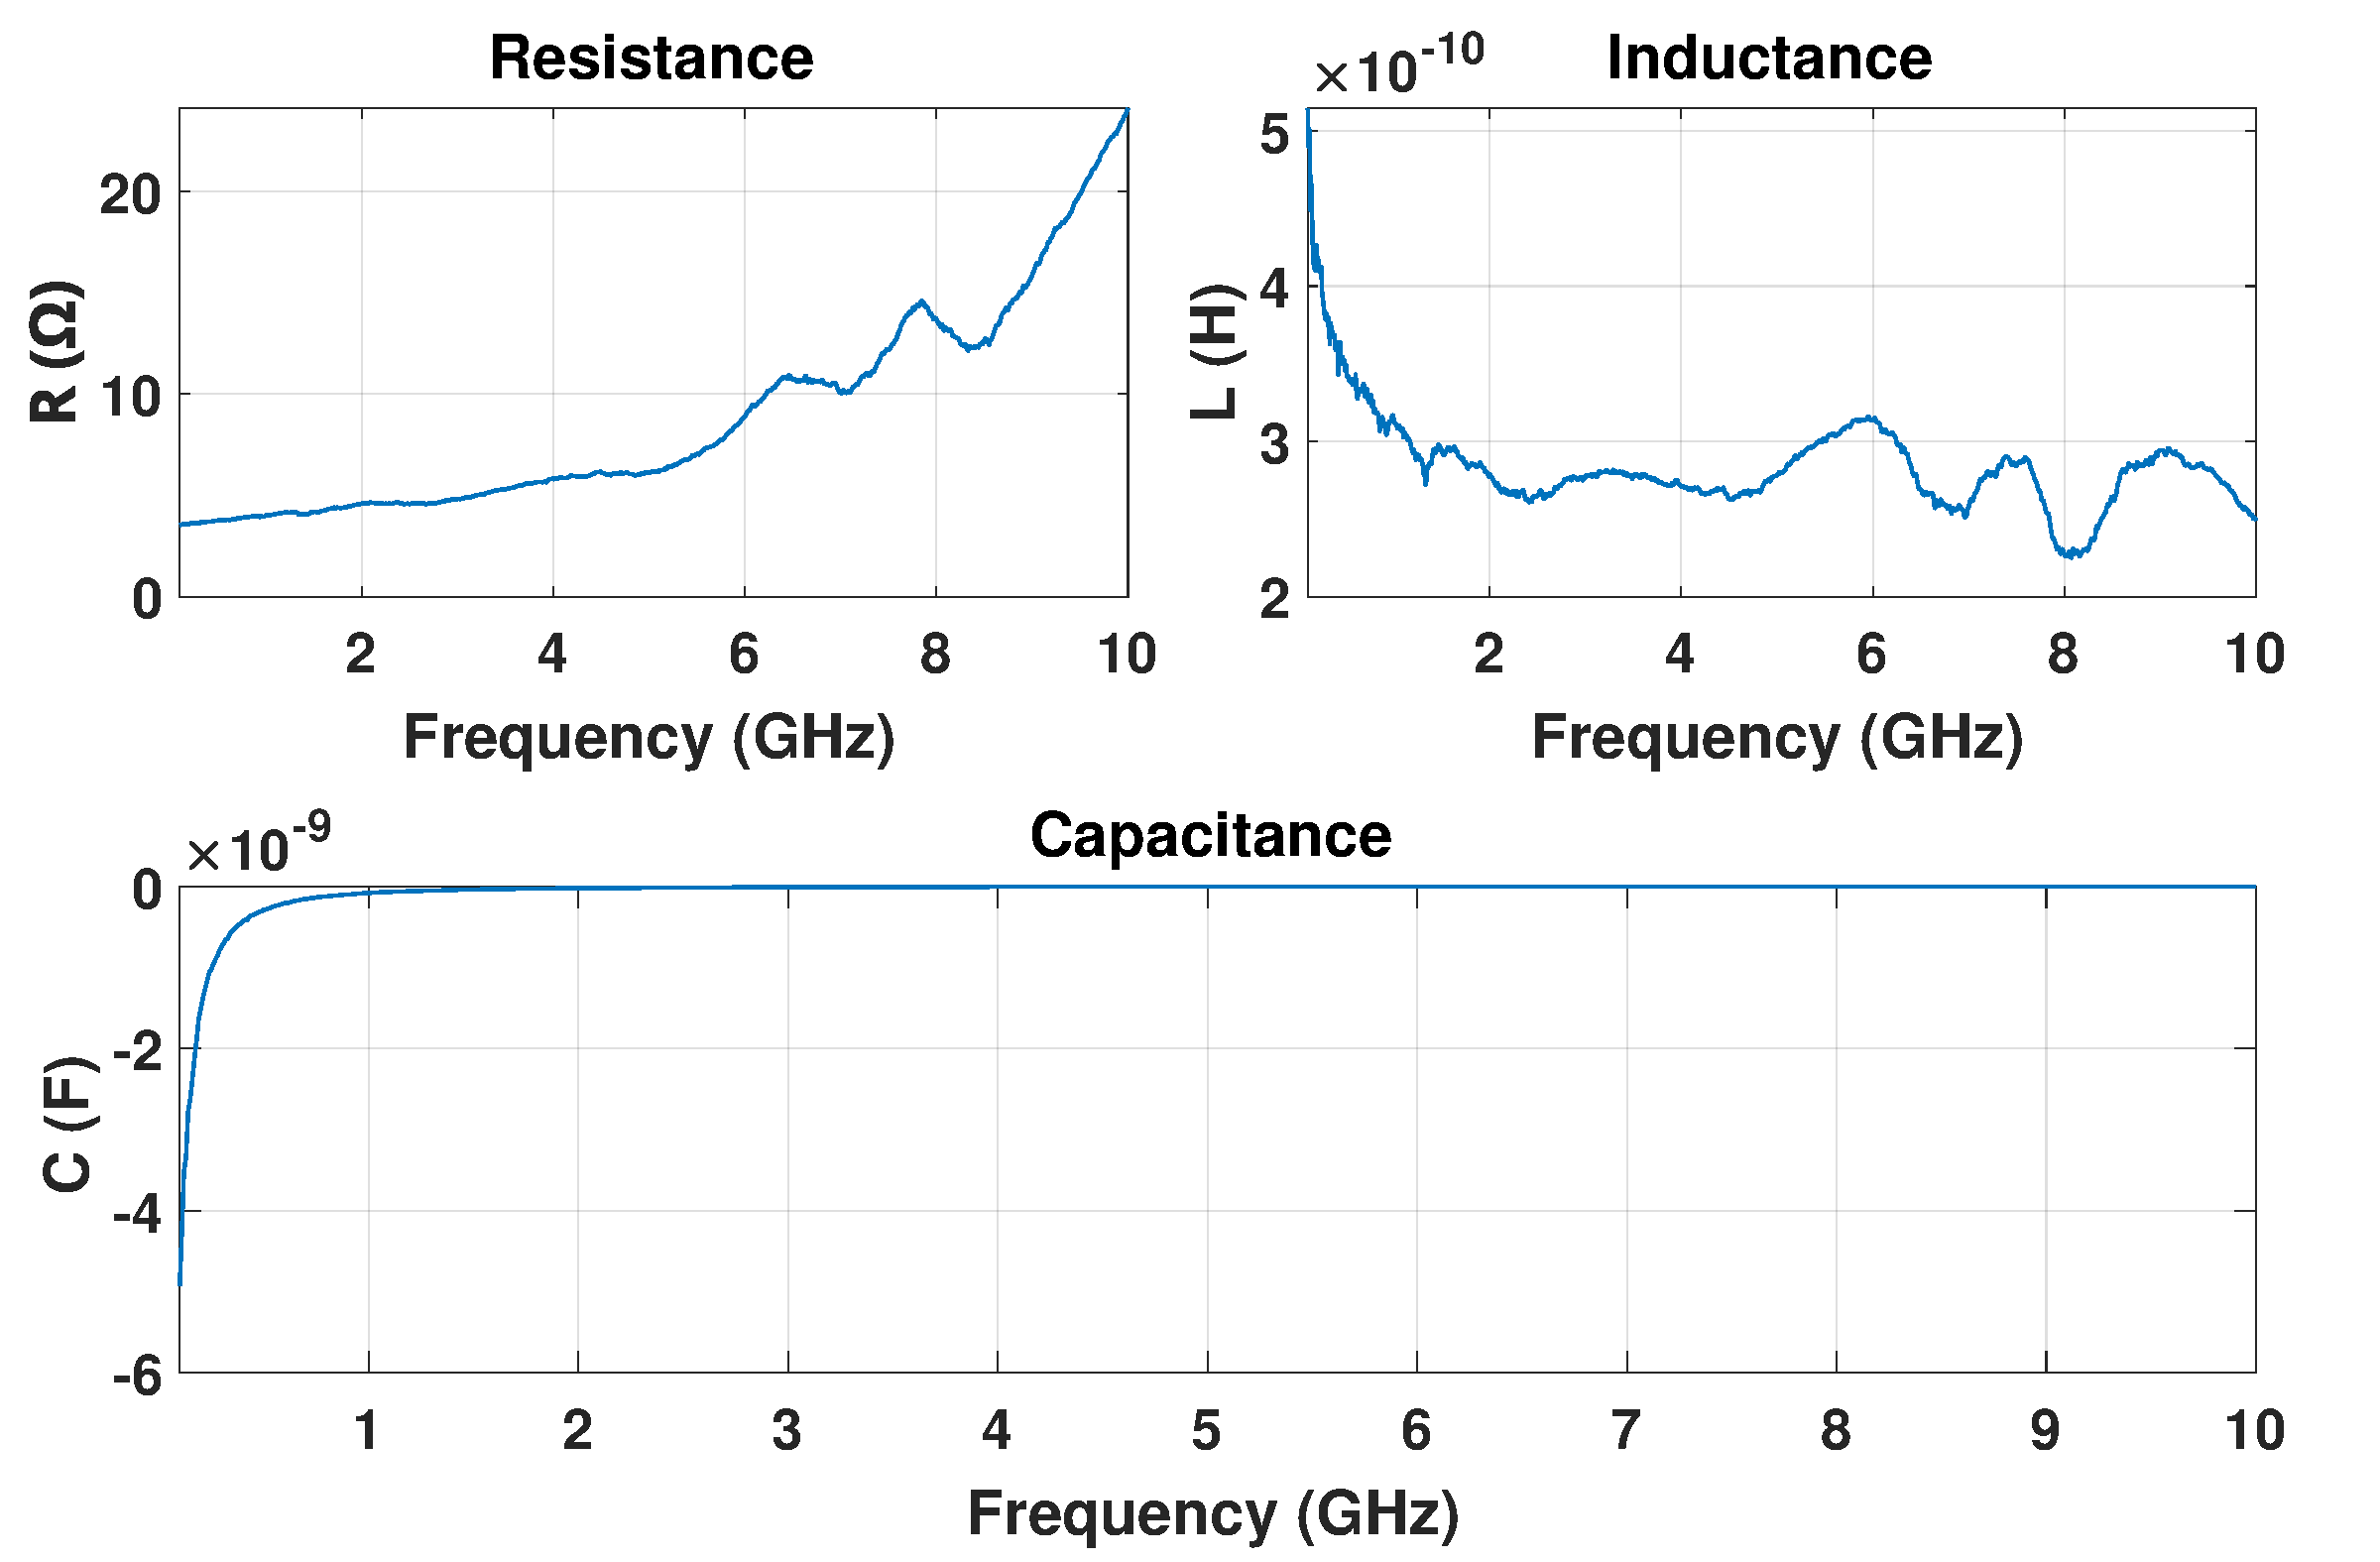
\includegraphics[width=\linewidth]{figures/RLC_finlaist.pdf}
  \caption{Extracted RLC parameters of a single gold bump after de-embedding from \SI{10}{\mega\hertz} to \SI{10}{\giga\hertz}.}
  \label{fig:rlc_bump}
  \vspace{-10px}
\end{figure}


\begin{figure}[htbp]
\vspace{-20px}
  \centering
  \begin{minipage}[t]{0.55\linewidth}
    \centering
    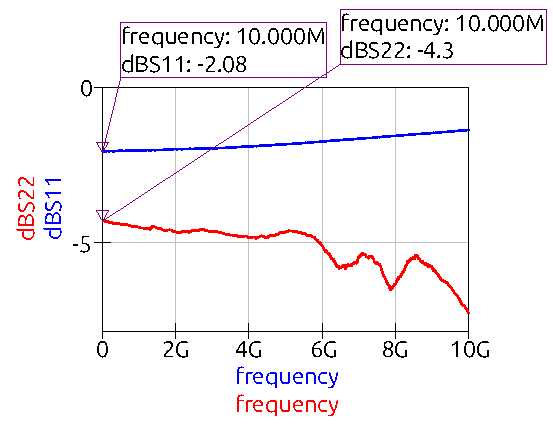
\includegraphics[width=\linewidth]{figures/rf_simulated_vs_real_dut_cropped_magnitude2.pdf}\\[-0.3em]
    (a)
  \end{minipage}\hfill
  \begin{minipage}[t]{0.42\linewidth}
    \centering
    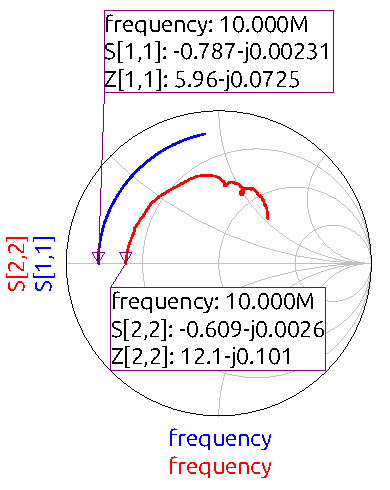
\includegraphics[width=\linewidth]{figures/rf_simulated_vs_real_dut_cropped_smithchart2.pdf}\\[-0.3em]
    (b)
  \end{minipage}
  \caption{Simulated (blue) versus measured (red) $S_{11}$ (\textsc{qucs} model) and
 $S_{22}$ of the real die + 3-bump + GSG system:
  Smith-chart (a) and magnitude (b).}
  \label{fig:sim_real}
  \vspace{-8px}
\end{figure}


\subsection{Yield Result Evaluation}\label{subsec:yield_res}

Fig.~\ref{fig:yield_die_res} labels the 24 lines on the
dummy die; Fig.~\ref{fig:yield_int_res} shows the corresponding
interposer.  
Two lines (\#17,\#22) were excluded because the lines were broken during fabrication, leaving \(N=22\) usable lines.  
Visual inspection and ohmic probing revealed
\(M_{\text{op}}=3\) open circuits,
\(M_{\text{sh}}=2\) shorts, and a single deformed bump that caused a short during the flip-chip, so the total defective count is \(M=6\).

Step\,1: fraction of defective chains
\begin{equation}
\Lambda = \frac{M}{N}= \frac{6}{22}=0.273.
\label{eq:lambda_meas}
\end{equation}

Step\,2: defective-bond probability
(with \(L=2\) bumps per chain)
\begin{equation}
\lambda = -\frac{1}{2}\ln\!\bigl(1-\Lambda\bigr)=0.159.
\label{eq:lambda_calc}
\end{equation}

Step\,3: single-bump yield
\begin{equation}
Y_{\text{bump}} = 1-\lambda = 0.841 \approx 84\,\%.
\label{eq:yield_84}
\end{equation}

The \SI{84}{\percent} bump yield is within the
\SIrange{80}{90}{\percent} window reported in a comparable thermosonic Au/Au bonding \cite{Ullan2004}.

\subsection{Final Discussion and Outlook}\label{subsec:final_discussion}
Although the single-metal Ti/Au glass interposer with \SI{70}{\micro\metre} Au studs achieves predictable \SI{10}{\mega\hertz}–\SI{10}{\giga\hertz} performance and an 84\% yield, its \SI{3.4}{\ohm} bump resistance, single-layer routing, and low-frequency model validity remain constraints in need of further validation. Future work is suggested to implement the gained process and data knowledge to enable cost-effective RF SiP prototypes on glass substrates such as those mentioned in appendix \ref{sec:appendix}. An extended version of this work will be submitted for publication.


\begin{figure}[htbp]
  \centering
  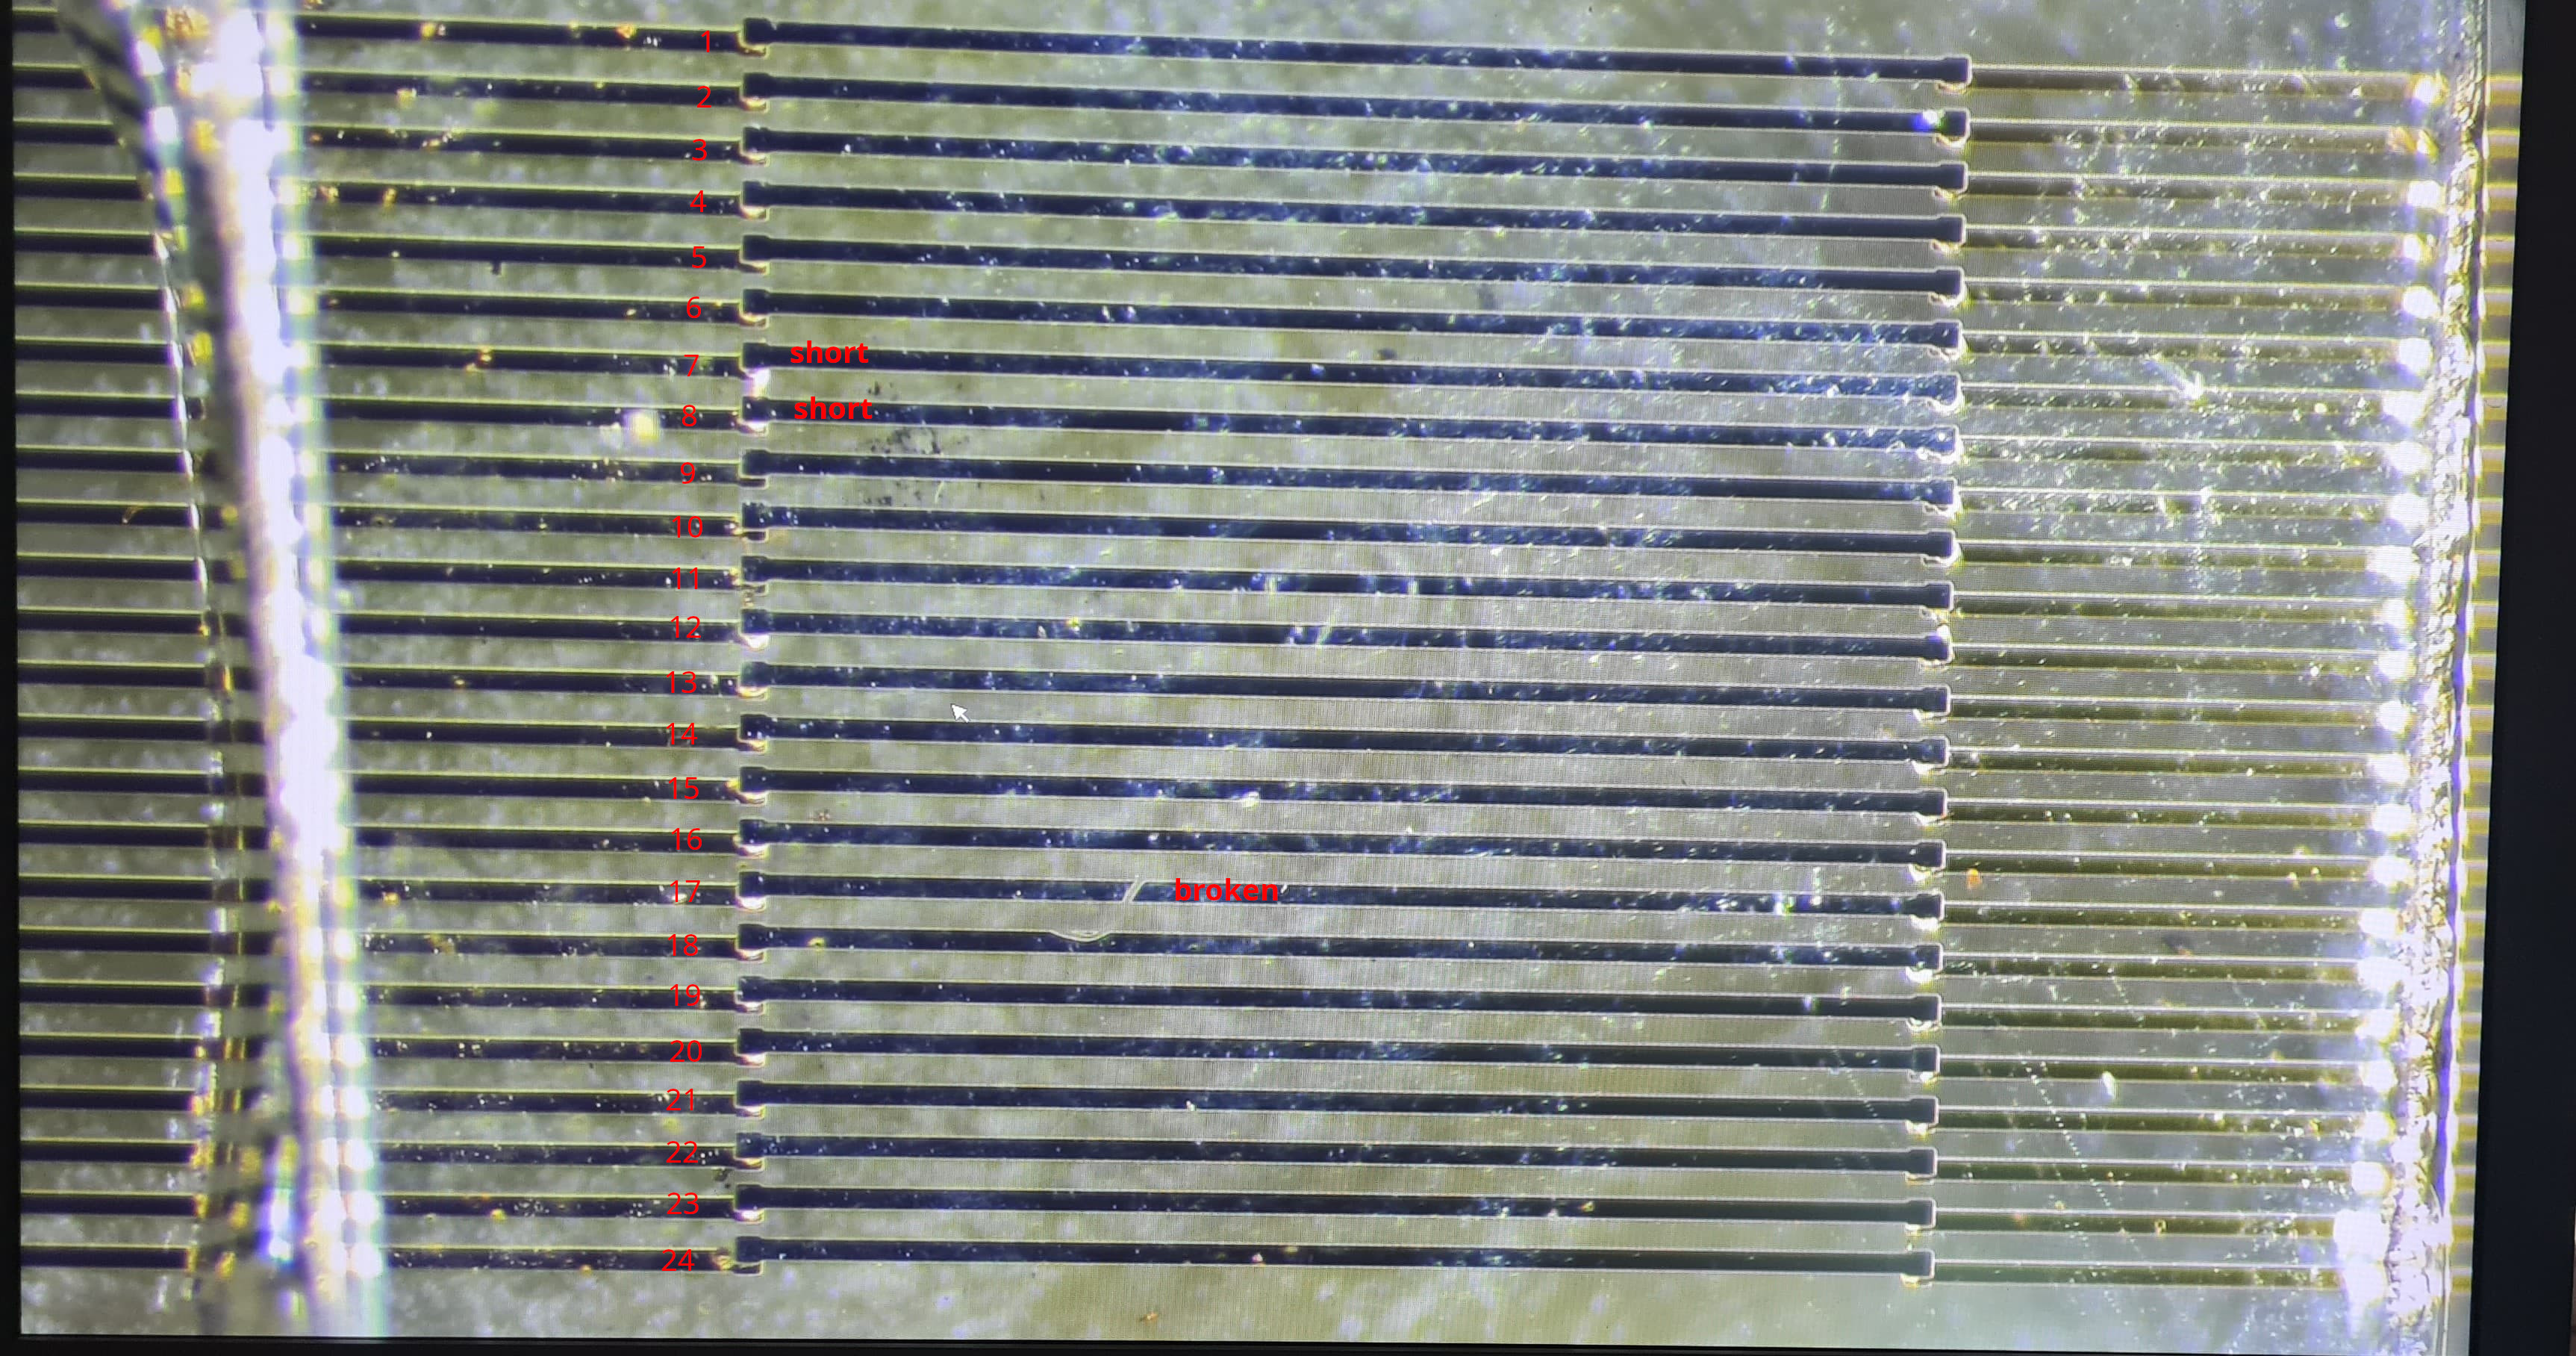
\includegraphics[width=\linewidth]{figures/yield_die.jpeg}
  \caption{Dummy die defects: lines 7–8 are shorted and 17 broken.}
  \label{fig:yield_die_res}
  \vspace{-10px}
\end{figure}

\begin{figure}[htbp]
  \centering
  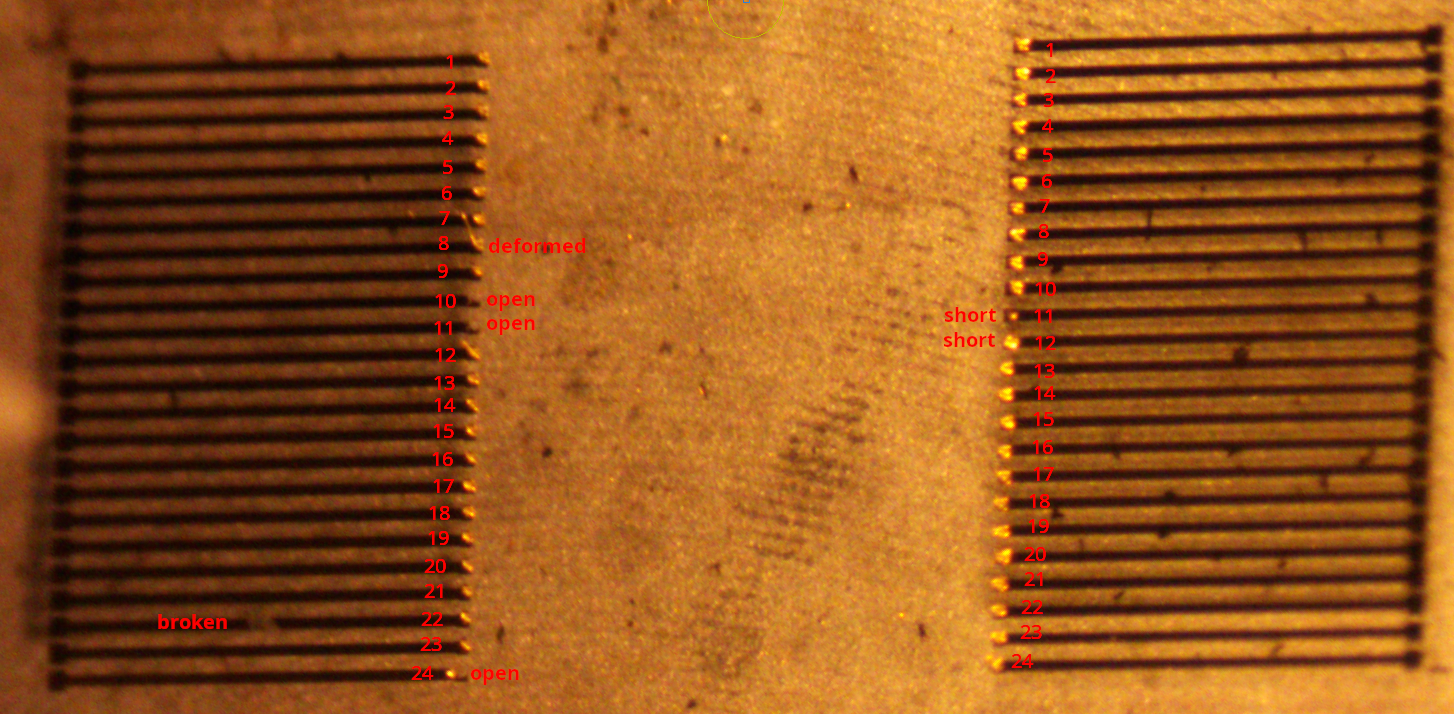
\includegraphics[width=\linewidth]{figures/yield_interposer.png}
  \caption{Interposer for yield analysis and defect annotation}
  \label{fig:yield_int_res}
  \vspace{-10px}
\end{figure}


\section{Conclusion}
A complete laboratory-grade flow for single-layer Ti (50 nm)/Au (100 nm) GSG flip-chip interposers on glass has been demonstrated and experimentally verified up to \SI{10}{GHz}.  The closed-form \(\pi\)-model for a \SI{1.15}{mm} CPWG (\(R=5.54\;\Omega,\,L=0.486\;\text{nH},\,C=66.1\;\text{fF}\)) agrees with VNA measurements to within 3 \%, while de-embedding shows each \SI{70}{\micro\metre} Au stud behaves as a \SI{3.4}{\ohm} series resistor at \SI{10}{MHz}.  Of 22 interconnect lines, after gold bump placement and thermo-compression flip-chip bonding, 84 \% yield was produced, confirming the robustness of the process. All masks, bonding parameters, and S-parameter data are included to enable full replication and extension of these results.

\begin{thebibliography}{1}
\bibitem{Lau2016}
J.~H.~Lau, Recent advances and new trends in flip chip technology,'' \emph{Journal of Electronic Packaging}, vol.~138, no.~3, pp.~030802, Jul. 2016.

\bibitem{Heinrich2005}
W.~Heinrich, 
Flip-chip for millimeter-wave and broadband packaging,'' 
in \emph{Proc. 2005 IEEE Int. Workshop Radio-Frequency Integration Technol. (RFIT)}, Singapore, 2005, pp.~124--126.

\bibitem{Keech2013}
J.~Keech, G.~Piech, S.~Pollard, S.~Chaparala, A.~Shorey, and B.~K.~Wang, 
Glass interposer substrates: Fabrication, characterization and modeling,'' 
in \emph{Proc. 15th IEEE Electron. Packag. Technol. Conf. (EPTC)}, Singapore, 2013, pp.~706--709.
\bibitem{Chang2022}
W.~Chang, Q.~Lu, J.~Zhang, W.~Xiang, C.~Zhu, M.~Zhao, and H.~Ye,  
``Optimization of micro-interconnection distribution of gold stud bumps for thermo-sonic flip chip bonding,''  
in \emph{Proc. 23rd Int. Conf. Electron. Packag. Technol. (ICEPT)}, Dalian, China, 2022, pp.~1--4.

\bibitem{Yan2024}
S.~Yan, L.~Zhao, Z.~Song, R.~Li, Y.~Hao, and Z.~Zhang, 
``A high-reliability Au stud bump bonding strategy based on Au pads for flip-chip bonding applications,'' 
in \emph{Proc. 9th Int. Conf. Integr. Circuits Microsyst. (ICICM)}, Nanjing, China, 2024, pp.~339--343.

\bibitem{Li2024}
F.~Li,  
``Flip-chip bonding for SiC integrated circuits with gold stud bumps for high temperature up to 600°C applications,''  
\emph{IEEE Trans. Components, Packag. Manuf. Technol.}, vol.~14, no.~4, pp.~705--713, Apr. 2024.

\bibitem{Simons2004}
R.~N.~Simons,  
\emph{Coplanar Waveguide Circuits, Components, and Systems}.  
Hoboken, NJ, USA: John Wiley \& Sons, 2004.

\bibitem{Wang2016}
H.~Wang, X.~Ren, J.~Zhou, \emph{et al.}, 
High frequency characterization and analysis of through silicon vias and coplanar waveguides for silicon interposer,'' 
\emph{Microsyst. Technol.}, vol.~22, pp.~337--347, Feb. 2016.

\bibitem{Ullan2004}
M.~Ullan, M.~Lozano, M.~Chmeissani, G.~Blanchot, E.~Cabruja, J.~Garcia, M.~Maiorino, R.~Martinez, G.~Pellegrini, and C.~Puigdengoles,  
Test chip for bump bond yield evaluation in high density flip chip technologies,''  
in \emph{Proc. IEEE Nucl. Sci. Symp. Conf. Rec.}, vol.~7, Rome, Italy, 2004, pp.~4347--4349.

\bibitem{Jordan2002}
J.~Jordan,  
Gold stud bump in flip-chip applications,''  
in \emph{Proc. 27th Annu. IEEE/SEMI Int. Electron. Manuf. Technol. Symp. (IEMT)}, San Jose, CA, USA, 2002, pp.~110--114.

\bibitem{Deng2016}
H.~Deng and Y.~Miao,  
Sapphire flip-chip thermocompression and eutectic bonding for dielectric laser accelerator,''  
Final Project Report, ENGR241, Stanford Univ., Stanford, CA, USA, Dec. 2016.

\bibitem{Makin1957}
S.~M.~Makin, A.~H.~Rowe, and A.~D.~Leclaire,  
``Self-diffusion in gold,''  
\emph{Proc. Phys. Soc. B}, vol.~70, no.~6, pp.~545--553, 1957.


\bibitem{Staiculescu2000}
D.~Staiculescu, J.~Laskar, and M.~Tentzeris,  
Flip chip design rule development for multiple signal and ground bump configurations,''  
in \emph{Proc. 2000 Asia-Pacific Microw. Conf. (APMC)}, Sydney, NSW, Australia, 2000, pp.~136--139.

\bibitem{Konstantinou2021}
D.~Konstantinou, C.~Caillaud, S.~Rommel, U.~Johannsen, and I.~Tafur Monroy,  
Investigation of de-embedding techniques applied on uni-traveling carrier photodiodes,''  
in \emph{Proc. 50th Eur. Microw. Conf. (EuMC)}, Utrecht, Netherlands, 2021, pp.~320--323.

\bibitem{Eisenstadt1992}
W.~R.~Eisenstadt and Y.~Eo,  
S-parameter-based IC interconnect transmission line characterization,''  
\emph{IEEE Trans. Components, Hybrids, Manuf. Technol.}, vol.~15, no.~4, pp.~483--490, Dec. 1992.

\bibitem{Basseri2018}
J.~Basseri, M.~Forouzanfar, R.~Feghhi, and M.~Joodaki,  
Design of X-band power amplifier based on the partitioning design approach,''  
in \emph{Proc. 26th Iranian Conf. Electr. Eng. (ICEE)}, Mashhad, Iran, May 2018, pp.~1--5.

\end{thebibliography}

\clearpage
\newpage

\section*{Appendix}\label{sec:appendix}

\subsection{Amplifier on Interposer Feasibility Study}\label{subsec:amp_feas}

After obtaining the research results of performing a successful flip-chip interposer bonding inside the TU/e lab facility, the next step is to apply the extracted knowledge and ideas onto a SiP feasibility study to extract maximum performance gain for something like a transistor that is meant to be used as an amplifier.

The \SI{5}{\giga\hertz} small signal benchmark for the common source TGF2023-2-02 GaN HEMT on an interposer was established by designing the mask-level common source amplifier layout that was later fabricated Fig.~\ref{fig:amp_masks}. Before implementing the design in \textsc{klayout} the simulation circuit was designed in \textsc{qucs} where the dimensions of the CPWG and passive components later accounted for when designing the mask were considered to achieve the best possible bias Fig.~\ref{fig:amp_schematic}. Compared with the resulting two-port S parameters with an ideal measurement of the bare die provided by the distributee of the chip, Fig.~\ref{fig:die_direct}-\ref{fig:die_extra_sparams}. The component choices mentioned in Table.~\ref{tab:passives} were calculated based on the bias network calculated in Table.~\ref{tab:calc} following the bias suggestions and the matched network research design strategy for the X band in \cite{Basseri2018}.

\begin{table}[htbp]
\caption{Surface-mount passives implemented on the interposer}
\label{tab:passives}
\begin{center}
\begin{tabular}{|c|c|c|}
\hline
\textbf{Ref.} & \textbf{Value / Rating} & \textbf{Package} \\
\hline
$R_S$ & \SI{22}{\ohm}, \SI{0.333}{W} & 0603 \\
$R_D$ & \SI{18}{\ohm}, \SI{0.333}{W} (opt.) & 0603 \\
$R_1$ & \SI{10}{\mega\ohm}, \SI{0.1}{W} & 0603 \\
$R_2$ & \SI{1}{\mega\ohm}, \SI{0.1}{W} & 0603 \\
$C_{1,2,3}$ & \SI{100}{\pico\farad}, \SI{50}{V}, NP0 & 0402 \\
$L_{\text{bias}}$ & \SI{4.7}{\micro\henry}, $I_\text{sat}=\SI{620}{mA}$ & 0603 \\
\hline
\end{tabular}
\end{center}
\end{table}

\begin{table}[htbp]
\caption{DC sizing at $V_{DD}=V_{DS}=\SI{28}{V}$, $I_{D}=\SI{128}{mA}$}
\label{tab:calc}
\begin{center}
\begin{tabular}{|c|c|c|}
\hline
\textbf{Quantity} & \textbf{Formula} & \textbf{Result} \\
\hline
$R_S$ & $V_S/I_D$ & \SI{21.9}{\ohm}\,$\rightarrow$\,\SI{22}{\ohm} \\
$P_{R_S}$ & $I_D^{2}R_S$ & \SI{0.36}{W} \\
$R_D$ & $(V_{DD}-V_D)/I_D$ & \SI{15.6}{\ohm}\,$\rightarrow$\,\SI{18}{\ohm} \\
$V_G$ & $V_{DD}R_2/(R_1+R_2)$ & \SI{2.55}{V} \\
$V_{GSQ}$ & $V_G-I_D R_S$ & \SI{-0.27}{V} \\
$L_{\text{bias}}$ margin & $I_{\text{sat}}\ge 2I_D$ & \SI{256}{mA} \\
\hline
\end{tabular}
\end{center}
\end{table}

Table.~\ref{tab:sparams} shows the key parameters extracted from the
simulations.  The interposer causes a \SI{1.9}{dB} reduction in forward gain (\(S_{21}\)).

\begin{table}[htbp]
\caption{Simulated $\mathbf{S}$-parameters at \SI{5}{GHz}}
\label{tab:sparams}
\begin{center}
\begin{tabular}{|c|c|c|}
\hline
 & \textbf{Die\,only} & \textbf{Die\,+\;interposer} \\
\hline
$|S_{21}|$ (dB) & $10.43$\, & $8.48$\, \\
$|S_{12}|$ (dB) & $-35.2$\, & $-7.78$\, \\
$Z_{11}$ (\si{\ohm}) & $2.8+j1.0$\ & $65.7+j35.5$\ \\
$Z_{22}$ (\si{\ohm}) & $21.4-j14.4$\ & $22.1+j36.0$\ \\
\hline
\end{tabular}
\end{center}
\end{table}

The amplifier case study serves a dual purpose in the context of previous research. First, it acts as system-level validation of the bump and line models extracted in section \ref{subsec:bump_line_model}. By embedding the \SI{70}{\micro\metre} gold‐bump transition and the single metal CPWG directly into the bias network Fig.~\ref{fig:amp_schematic} with its dimensions adjusted by considering the sheet resistance of the Ti/Au layer that was extracted in section \ref{subsec:rlcg}, the simulation reproduces the expected \SI{\sim2}{\dB} gain penalty seen when moving from directly probing the die to a fully packaged on interposer circuit Table.~\ref{tab:sparams}. Second, the study demonstrates the practical design advantage that a single-layer glass interposer can offer for active RF functions. The simulated common-source amplifier maintains the gain that can be used for signal amplification until \SI{5} {\giga\hertz}.

\begin{figure}[htbp]
  \centering
  \begin{minipage}[t]{0.49\linewidth}
    \centering
    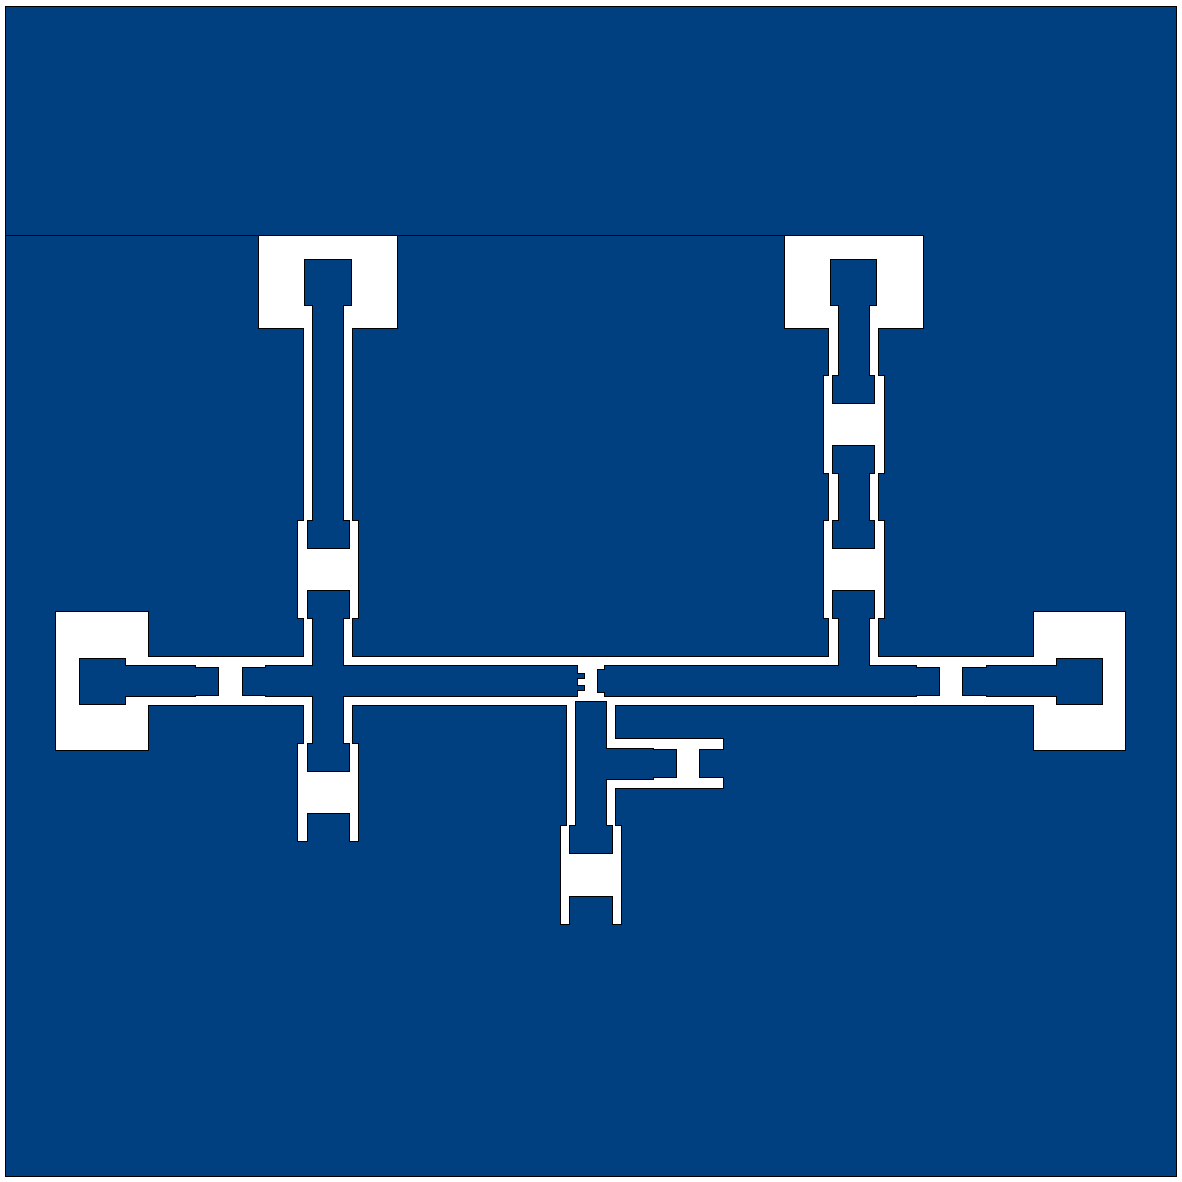
\includegraphics[width=\linewidth]{figures/amplifier_layout_passive.png}\\[-0.2em]
    (a)
  \end{minipage}\hfill
  \begin{minipage}[t]{0.49\linewidth}
    \centering
    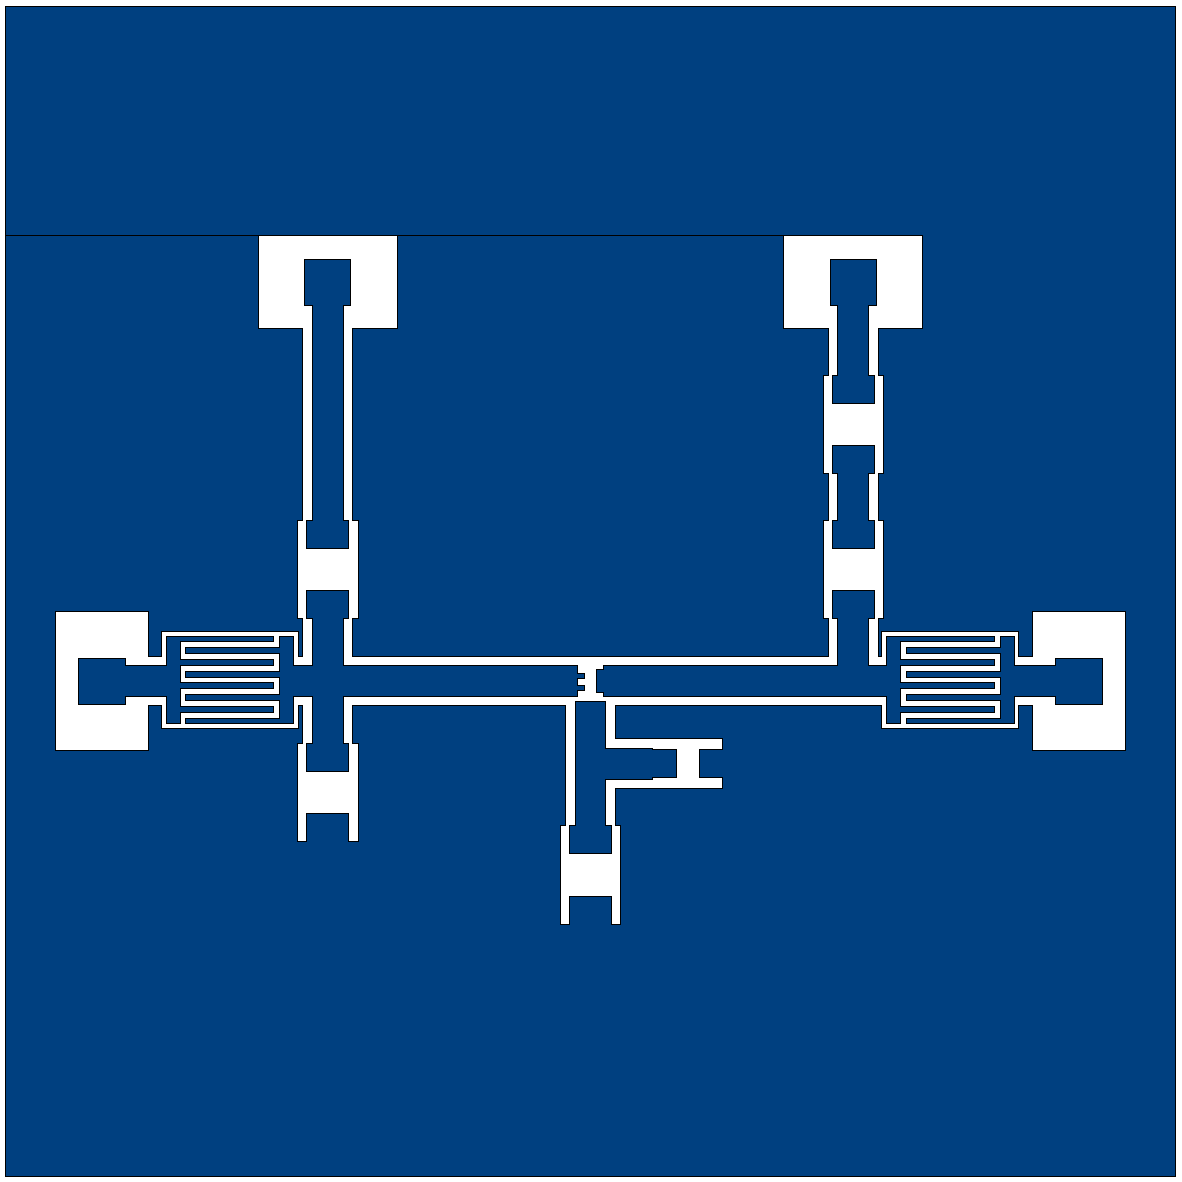
\includegraphics[width=\linewidth]{figures/amplifier_layout_planar.png}
    (b)
  \end{minipage}
  \caption{Mask options for the common-source amplifier:
  (a) discrete DC blocks, (b) planarised DC blocks.}
  \label{fig:amp_masks}
\end{figure}

\begin{figure}[htbp]
  \centering
  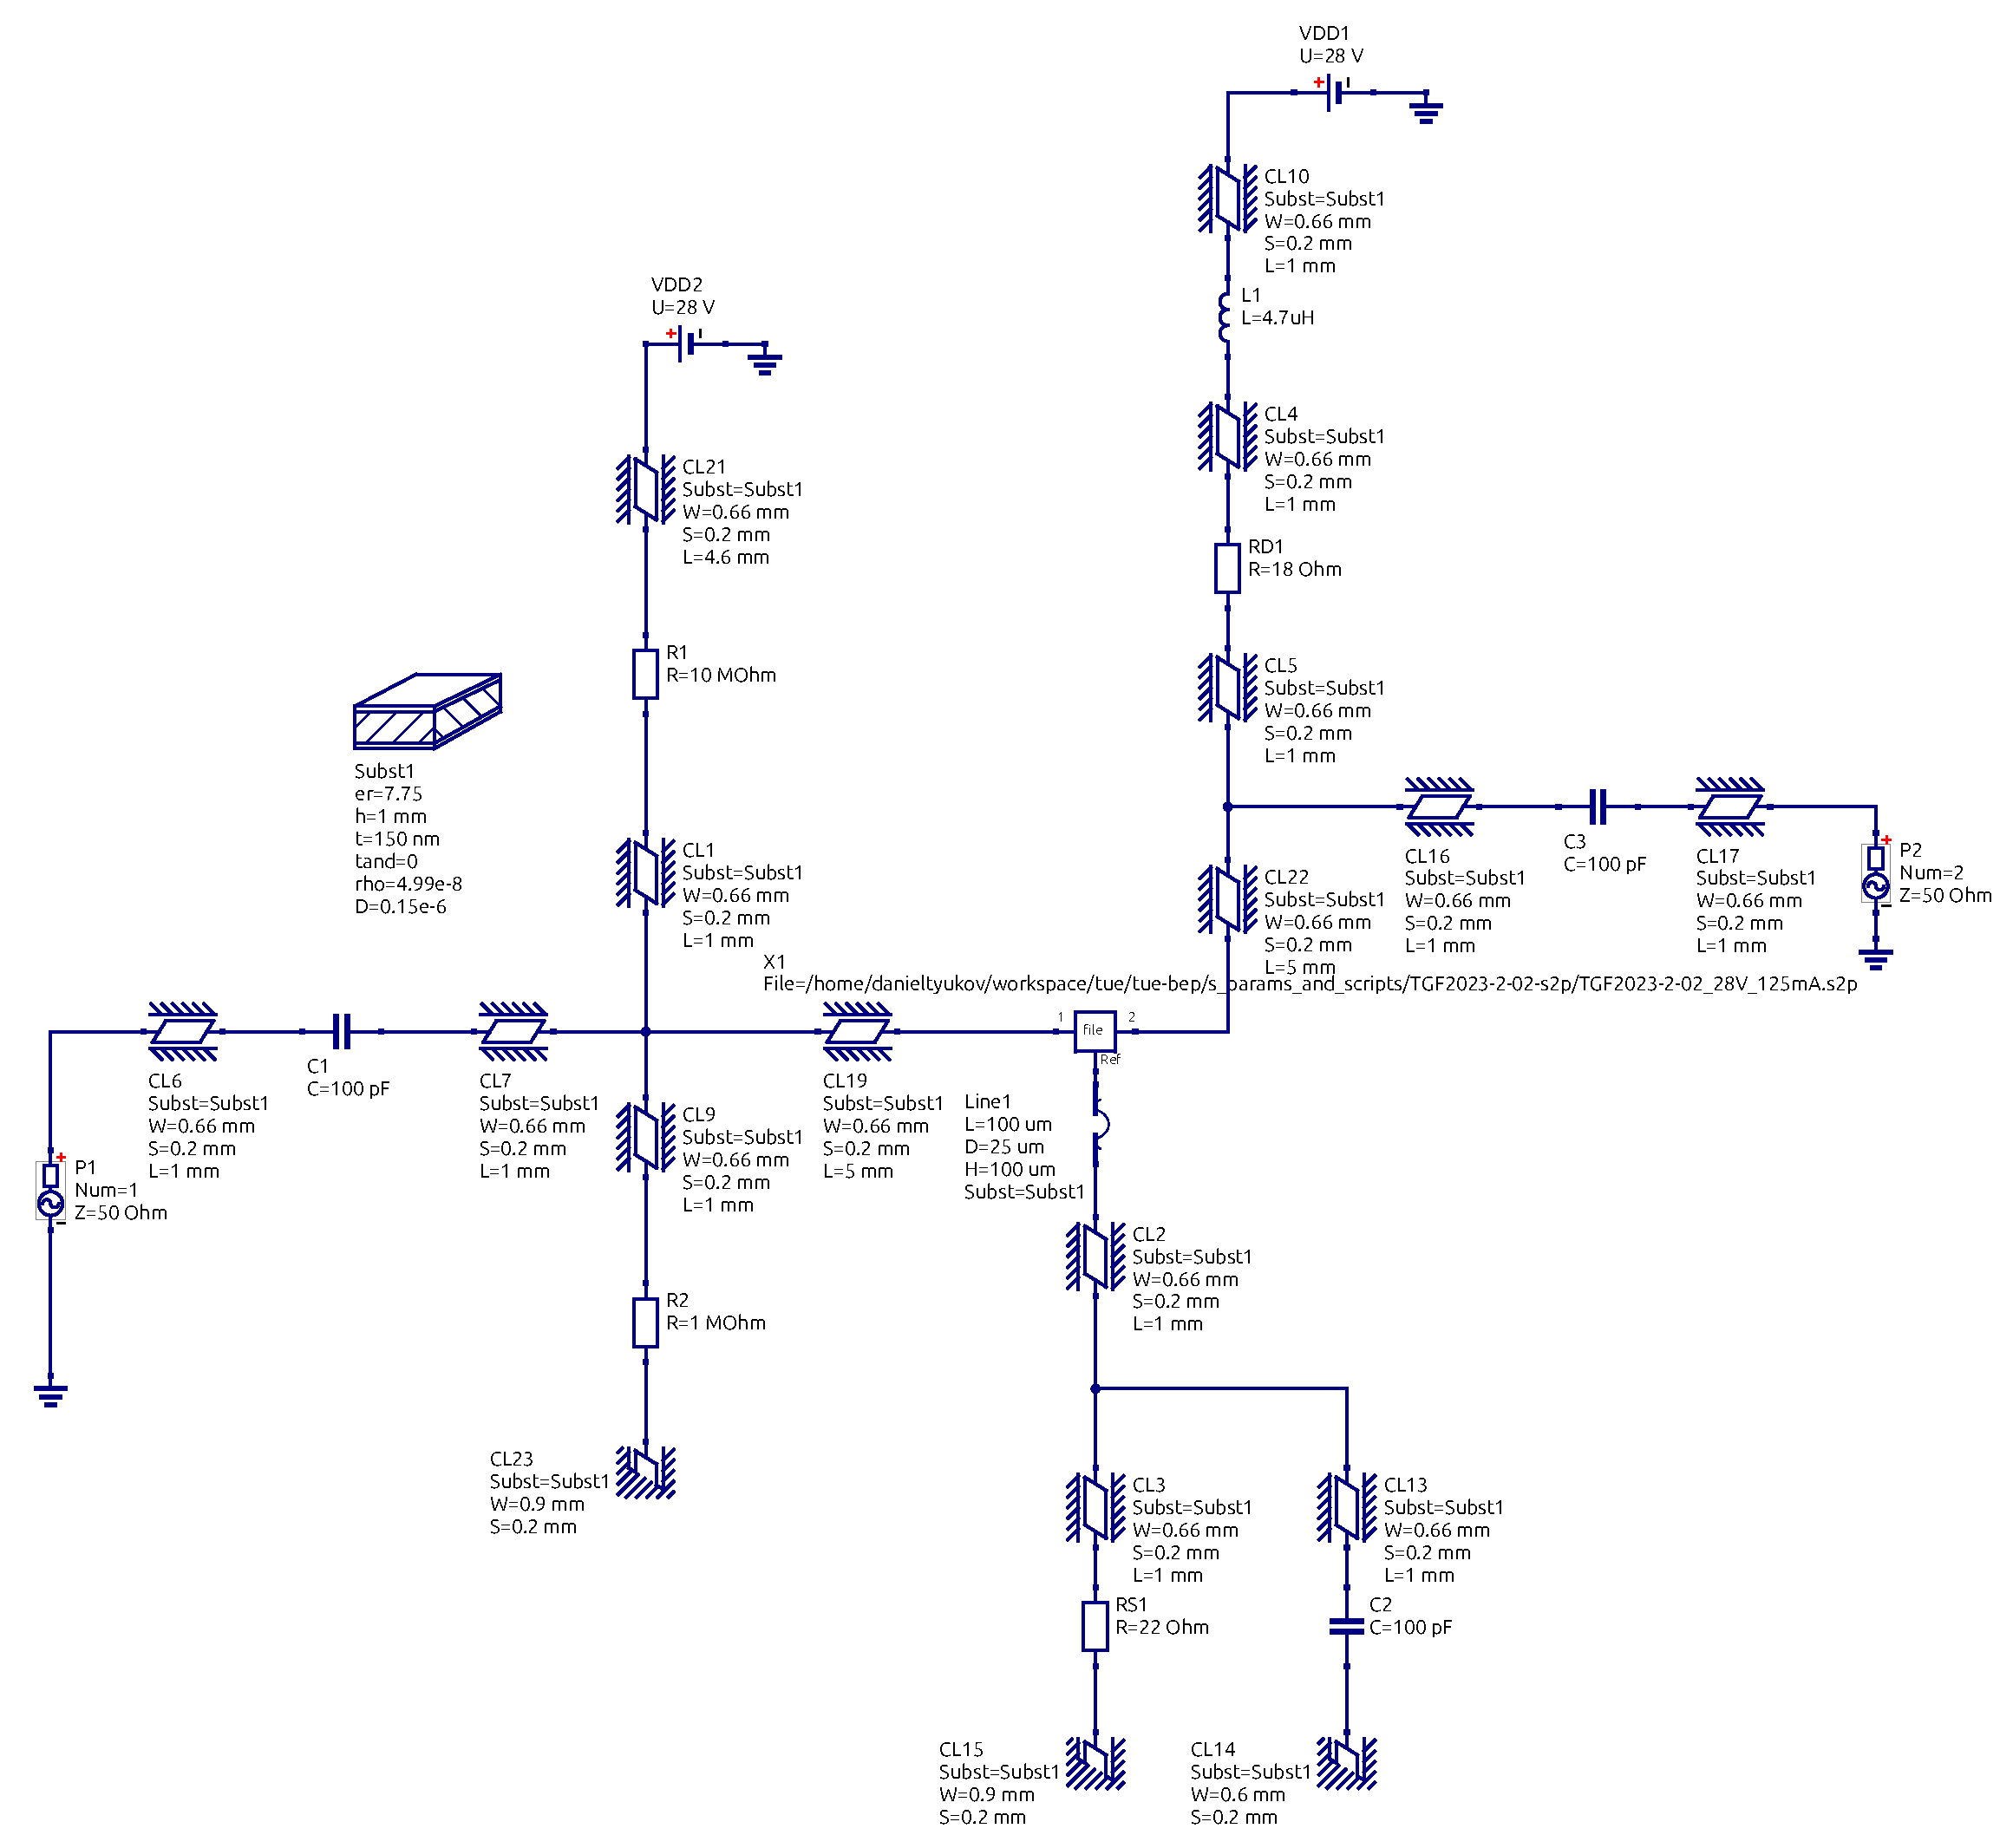
\includegraphics[width=\linewidth]{figures/tgf_2023_2_02_cw_model.pdf}
  \caption{\textsc{qucs} schematic of the amplifier, indicating CPWG
  sections and bias voltage.}
  \label{fig:amp_schematic}
\end{figure}

\begin{figure}[htbp]
  \centering
  \begin{minipage}[t]{0.49\linewidth}
    \centering
    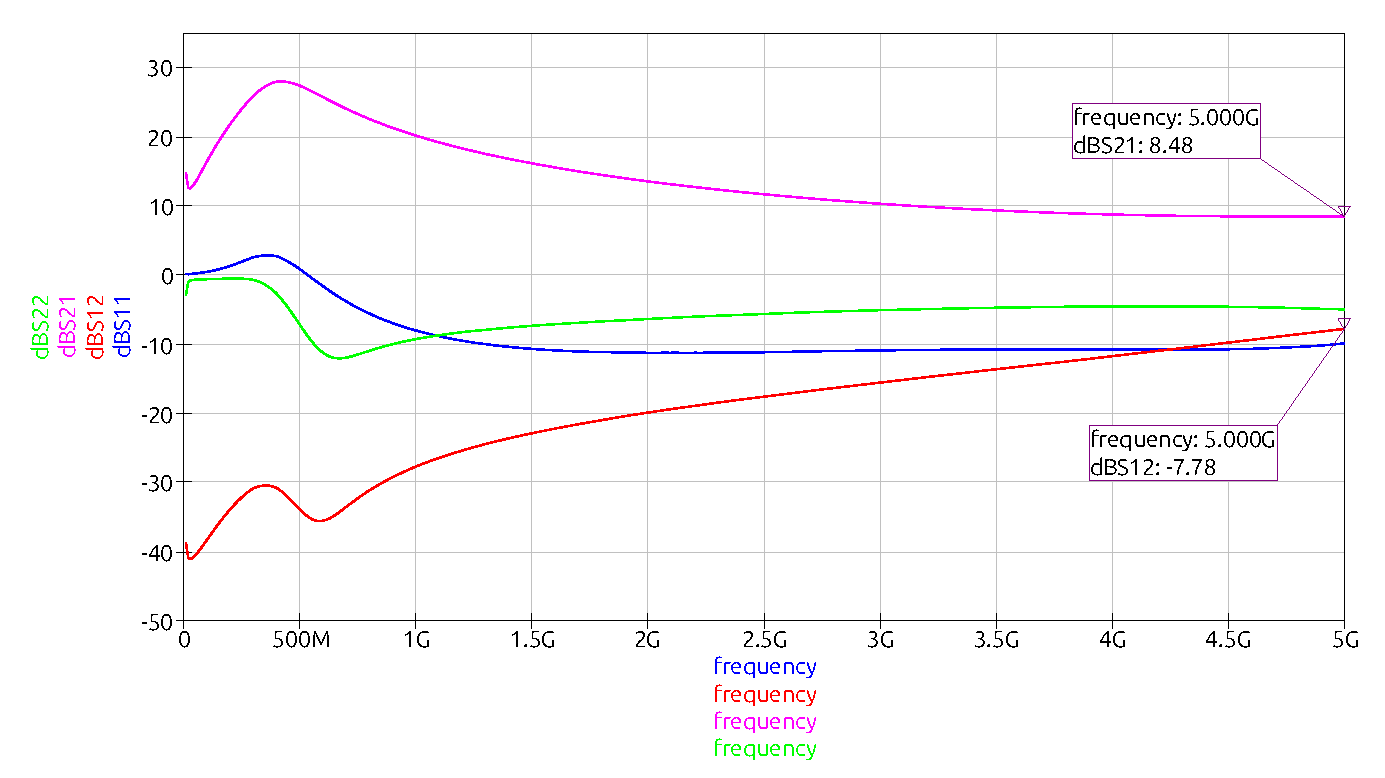
\includegraphics[width=\linewidth]{figures/tgf_2023_2_02_cw_model_g1.pdf}\\[-0.25em]
    (a)
  \end{minipage}\hfill
  \begin{minipage}[t]{0.49\linewidth}
    \centering
    
\includegraphics[width=\linewidth]{%
      figures/tgf_2023_2_02_cw_model_g2.pdf}\\[-0.25em]
    (b)
  \end{minipage}
  \caption{Simulated amplifier response:
  (a) $|S_{21}|$ magnitude, (b) Smith-chart view of $S_{11}$/$S_{22}$.}
  \label{fig:amp_model_sparams}
\end{figure}

\begin{figure}[htbp]
  \centering
  \begin{minipage}[t]{0.49\linewidth}
    \centering
    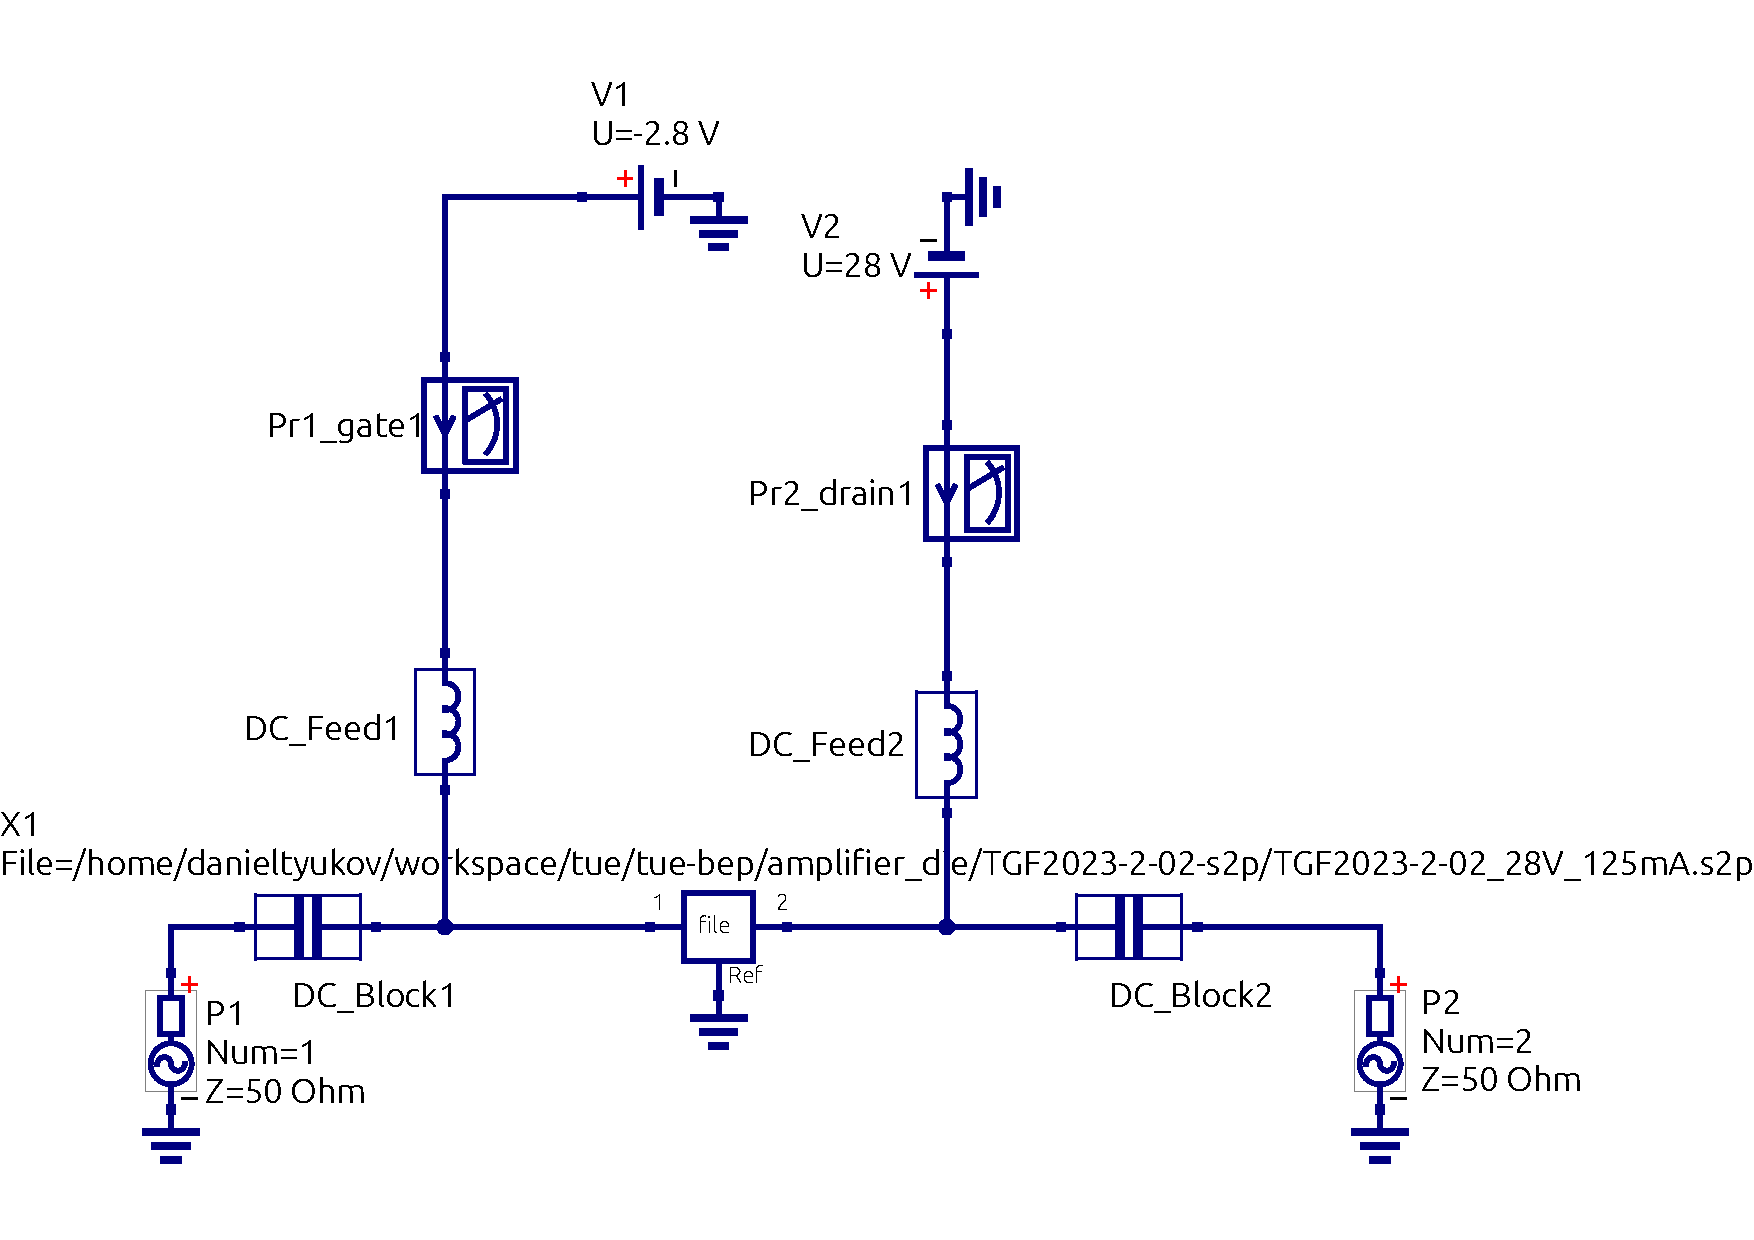
\includegraphics[width=\linewidth]{figures/tgf_2023_2_02_cw_test_model.pdf}\\[-0.25em]
    (a)
  \end{minipage}\hfill
  \begin{minipage}[t]{0.49\linewidth}
    \centering
    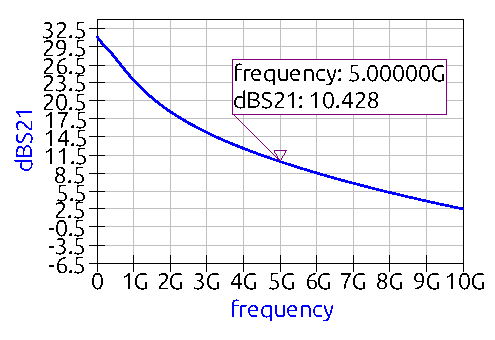
\includegraphics[width=\linewidth]{figures/tgf_2023_2_02_cw_test_model_g1.pdf}\\[-0.25em]
    (b)
  \end{minipage}
  \caption{Die-only characterization reference:
  (a) direct-test schematic, (b) measured $|S_{21}|$ magnitude.}
  \label{fig:die_direct}
\end{figure}

\begin{figure}[htbp]
  \centering
  \begin{minipage}[t]{0.32\linewidth}
    \centering
    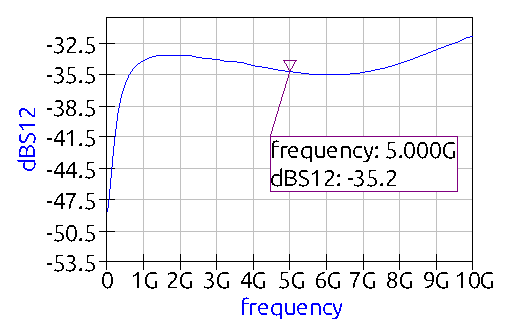
\includegraphics[width=\linewidth]{figures/tgf_2023_2_02_cw_test_model_g2.pdf}\\[-0.4em]
    (a)
  \end{minipage}\hfill
  \begin{minipage}[t]{0.32\linewidth}
    \centering
    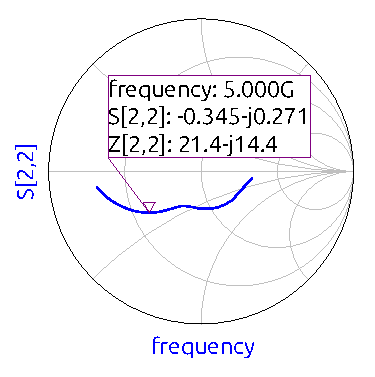
\includegraphics[width=\linewidth]{figures/tgf_2023_2_02_cw_test_model_g3.pdf}\\[-0.4em]
    (b)
  \end{minipage}\hfill
  \begin{minipage}[t]{0.32\linewidth}
    \centering
    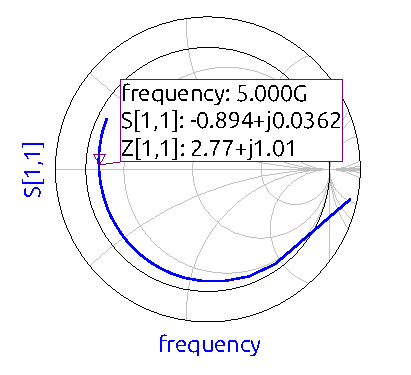
\includegraphics[width=\linewidth]{figures/tgf_2023_2_02_cw_test_model_g4.pdf}\\[-0.4em]
    (c)
  \end{minipage}
  \caption{Additional die-only measurements:
  (a) $|S_{12}|$ magnitude,
  (b) Smith-chart $S_{11}$,
  (c) Smith-chart $S_{22}$.}
  \label{fig:die_extra_sparams}
\end{figure}


\end{document}